\documentclass[12pt,a4paper,pdftex,final,oneside,titlepage]{book}
\usepackage[pdftex]{graphicx,color}
\usepackage{graphicx}
\usepackage[left=4cm,top=3cm,right=3cm,bottom=3cm,includeheadfoot]{geometry} %untuk mengatur margin
\usepackage[pdftex]{hyperref}
\usepackage{lscape}
%\begin{landscape} untuk awal landsacpe
%landscape content
%\end{landscape} untuk akhir landscape
\usepackage{longtable}
\usepackage{setspace} %untuk mengatur spasi, pilihan: \doublespacing \singlespacing atau \onehalfspacing   
\usepackage[bahasa]{babel}
\selectlanguage{bahasa}
\usepackage{fancyhdr,lastpage}
%\usepackage[Lenny]{fncychap}
%\usepackage[Sonny]{fncychap}
\usepackage{pstricks}
\usepackage{listings} %listing program
\usepackage{appendix}
\usepackage{subfig} %sub figure
\usepackage{sidecap} %side caption
\usepackage{ulem} %striketrough

%==========================================================================================================
% Bagian konfigurasi listing code
%========================================================================================================== 

% Colors used by Flex Builder 3.
\definecolor{purple}{rgb}{0.65, 0.12, 0.82}
\definecolor{flexred}{rgb}{0.65, 0.01, 0.01}
\definecolor{flexgreen}{rgb}{0, 0.6, 0}
\definecolor{flexgray}{rgb}{0.25, 0.37, 0.75}
\definecolor{flexblue}{rgb}{0, 0.2, 1}
\definecolor{flexfunction}{rgb}{0.2, 0.6, 0.4}
\definecolor{flexvar}{rgb}{0.4, 0.6, 0.8}
\definecolor{light-gray}{gray}{0.93}

% Define new language for listings.
\lstdefinelanguage{ActionScript} {
	basicstyle=\ttfamily\scriptsize,
	sensitive=true,
	morecomment=[l][\color{flexgreen}\ttfamily]{//},
	morecomment=[s][\color{flexgreen}\ttfamily]{/*}{*/},
	morecomment=[s][\color{flexgray}\ttfamily]{/**}{*/},
	morestring=[b]",
	stringstyle=\color{flexred}\textbf,
	commentstyle=\color{flexgreen},
	showstringspaces=false,
	numberstyle=\scriptsize,
	numberblanklines=true,
	showspaces=false,
	breaklines=true,
	showtabs=false,
	xleftmargin=17pt,
    framexleftmargin=17pt,
    framexrightmargin=5pt,
    framexbottommargin=4pt,
    backgroundcolor=\color{light-gray},
	emph =
	{[1]
		class, package, interface
	},
	emphstyle={[1]\color{purple}\textbf},
	emph =
	{[2]
		internal, public, protected, private,
		super, this, import, new, extends, implements,
		void, true, false, as
	},
	emphstyle={[2]\color{flexblue}\textbf},
	emph =
	{[3]
		function
	},
	emphstyle={[3]\color{flexfunction}\textbf},
	emph =
	{[4]
		var
	},
	emphstyle={[4]\color{flexvar}\textbf}
}

% Define new language for listings.
\lstdefinelanguage{MXML} {
   basicstyle=\ttfamily\scriptsize,
   sensitive=true,
   morecomment=[s][\color{flexred}\ttfamily]{<!--}{-->}, commentstyle=\color{flexred},
   morecomment=[s][\color{black}]{<?}{?>}, commentstyle=\color{black},
%  morecomment=[n][\color{black}]{\{}{\}}, commentstyle=\color{black},
   string=[b]", stringstyle=\color{flexred},
   morestring=[b]', stringstyle=\color{flexred},
   showstringspaces=false,
   numberstyle=\scriptsize,
   numberblanklines=true,
   showspaces=false,
   breaklines=true,
   showtabs=false,
   alsoletter={:},
   keywords = [1]
   {
      mx:WindowedApplication, mx:Application, mx:Button, mx:Text,
      mx:HBox, mx:VBox
   },
   keywordstyle={[1]\color{flexblue}},
%  otherkeywords={<,>,/>,</},
   keywords = [2]
   {
      mx:Script
   },
   keywordstyle={[2]\color{flexgreen}},
}

\DeclareCaptionFont{white}{\color{white}}
\DeclareCaptionFormat{listing}{\colorbox{gray}{\parbox{\textwidth}{#1#2#3}}}
\captionsetup[lstlisting]{format=listing,labelfont=white,textfont=white}


%\makeatletter
%\newcommand\appendix@chapter[1]{%
%  \refstepcounter{chapter}%
%  %\orig@chapter*{Lampiran \@Alph\c@chapter #1}%
%  \addcontentsline{toc}{chapter}{Lampiran \@Alph\c@chapter: #1}%
%}
%\g@addto@macro\appendix{\let\chapter\appendix@chapter}
%\makeatother
%
%\makeatletter
%\newcommand\appendix@section[1]{%
%  \refstepcounter{section}%
%  \addcontentsline{toc}{section}{\@Alph\c@section: #1}%
%}
%\makeatother


%==========================================================================================================
% Bagian input data untuk keterangan file PDF yang dihasilkan
%========================================================================================================== 
\pdfinfo{
/Author (Rizky Zulkarnaen)
/CreationDate (D:20100602300000) % D:YYYYMMDDhhmmss (diisi dengan tanggal pembuatan skripsi)
/ModDate (D:20100602300000) % diisi dengan tanggal modifikasi skripsi
/Creator (LaTeX)
/Producer (pdfLaTeX)
/Title (TA_AR) % diisi dengan nama file skripsi
/Subject (Perancangan Aplikasi Viewer Model 3D Interaktif Berbasis Web dengan Teknologi Augmented Reality) % diisi dengan judul skripsi
/Keywords (augmented reality, computer vision, 3D) % diisi dengan kata-kata kunci isi skripsi
}

%==========================================================================================================
% Bagian pengaturan hyperref
%========================================================================================================== 
\hypersetup{
pdftitle={Perancangan Aplikasi Viewer Model 3D Interaktif Berbasis Web dengan Teknologi Augmented Reality}, % diisi dengan judul akhir skripsi
pdfauthor={Rizky Zulkarnaen}, % diisi dengan nama penulis skripsi
pdfkeywords={augmented reality computer vision 3D}, % diisi dengan kata-kata kunci dari isi skripsi
bookmarksnumbered,
pdfstartview={FitH},
	citecolor = black,
	linkcolor=black,
  colorlinks
}

%==========================================================================================================
% Koleksi pemenggalan kata, isi bagian ini bisa ditambah jika Anda mendapati kata yang salah pemenggalannya 
%==========================================================================================================
\hyphenation{HTTP}
\hyphenation{client}
\hyphenation{dengan}
\hyphenation{header}
\hyphenation{lingkung-an}
\hyphenation{di-mung-kin-kan}
\hyphenation{trans-pa-ran}
\hyphenation{gen-era-tor}
\hyphenation{apli-kasi}
\hyphenation{me-nam-pil-kan}
\hyphenation{di-tamb-bah-kan}
\hyphenation{ber-da-sar-kan}
\hyphenation{da-pat}
\hyphenation{nya-ta}
\hyphenation{ge-ne-ra-tor}
\hyphenation{sua-tu}
\hyphenation{pe-ran-cang-an}
\hyphenation{di-tam-bah-kan}
\hyphenation{ci-tra}
\hyphenation{ka-li-be-ra-si}
\hyphenation{ber-dam-ping-an}
\hyphenation{FLAR-ToolKit}
\hyphenation{di-sa-ji-kan}
\hyphenation{mar-ker}
\hyphenation{di-ki-rim}
\hyphenation{me-nga-tur}
\hyphenation{ka-rak-ter-istik}
%==========================================================================================================
% Bagian pengaturan paragraf 
%==========================================================================================================
\setlength{\parindent}{0pt} % jika awal paragraf ingin dibuat menjorok ke dalam, ganti angka 0 nya. 
\setlength{\parskip}{6pt plus1pt minus1pt}
\newcommand{\marginal}[1]{\leavevmode\marginpar{\color{cyan}\footnotesize\raggedright#1\par}} 
\onehalfspacing
%==========================================================================================================
% Bagian pengaturan Fancy Header
%==========================================================================================================
\setlength{\headheight}{15pt}

%==========================================================================================================
% BAGIAN ISI DOKUMEN 
%==========================================================================================================
\begin{document}  

%==========================================================================================================
% Bagian pembuatan halaman judul 
%==========================================================================================================
\pagestyle{empty} 
	\begin{titlepage} 
		\begin{center} 
		{\Large\textbf{Bahan Seminar Tugas Akhir}}\\
		\par
		\vspace{2cm}
		\textbf{\Large Perancangan Aplikasi \textit{Viewer} Model 3D Interaktif Berbasis \textit{Web} dengan Teknologi \textit{Augmented Reality}} % diisi dengan judul skripsi
		\vspace{0.5cm} \\
		oleh :\\[0.4cm] 
		{\large\underline{Rizky Zulkarnaen}}\\
		$050402056$ \\% ganti NIM
		\end{center}
		
		\par
		\vfill
		
		\begin{figure}[h]
			\begin{center}
				
\includegraphics[width=4.2cm]{./images/logoUSU} % isi dengan nama file logo
			\end{center}
        \end{figure}
        
        \vfill 
        
      \begin{center}
      {\bf \large DEPARTEMEN TEKNIK ELEKTRO}\\[0.4cm] 
      {\bf \large FAKULTAS TEKNIK}\\[0.4cm] 
      {\bf \large UNIVERSITAS SUMATERA UTARA}\\[0.4cm] 
      {\bf \large MEDAN}\\[0.4cm] 
      {\bf \large 2010}
      \end{center}
      
   \end{titlepage} 

%==========================================================================================================
% Bagian pembuatan halaman pengesahan skripsi 
%==========================================================================================================
\thispagestyle{empty} 
\begin{center}{%\fontfamily{phv}\selectfont

\textbf{\large Perancangan Aplikasi \textit{Viewer} Model 3D Interaktif Berbasis \textit{Web} dengan Teknologi \textit{Augmented Reality}}\\[1cm] 

\par 
\vspace{0.4cm} 
oleh : 
\\
{\large\underline{Rizky Zulkarnaen}}\\ 
$050402056$
} 
\vspace{1.4cm} 

Tugas Akhir ini diajukan untuk melengkapi salah satu syarat untuk memperoleh gelar Sarjana Teknik\\[0.2cm] 

Disetujui oleh :\\ 
Pembimbing\\[2.2cm] 
\textbf{\bfseries \underline{Ori Novanda, MT}}\\[0.2cm] 
NIP:1972.1114.2003.121001\\[0.4cm]
Diketahui oleh :\\ 
Pelaksana Harian Ketua Departemen Teknik Elektro\\[2.2cm] 
\textbf{\bfseries \underline{Prof. Dr. Ir. Usman S. Baafai}}\\[0.2cm] 
NIP:1946.1022.1973.02001\\ 

\end{center} 
%========================================================================================================== 
% Bagian pengaturan header dan footer
%========================================================================================================== 
\pagestyle{fancy}
\lhead{} \chead{} \rhead{\thepage}
\lfoot{} \cfoot{} \rfoot{}
\renewcommand\headrulewidth{0pt}
\renewcommand\footrulewidth{0pt}

%==========================================================================================================
% ISI SKRIPSI 
%==========================================================================================================
\pagenumbering{roman}
\setcounter{tocdepth}{5} 
\setcounter{secnumdepth}{3} %ditambahkan agar perintah \subsubsection memiliki angka

%==========================================================================================================
%ABSTRAK
%==========================================================================================================

\chapter*{\centering Abstrak}
\thispagestyle{empty}
\addcontentsline{toc}{chapter}{Abstrak}
Dewasa ini, representasi model tiga dimensi (3D) virtual pada komputer sangat populer. Pemodelan model 3D virtual tersebut memerlukan interaksi yang baik dengan pengguna untuk mendapatkan sudut pandang yang jelas dari objek tersebut. Beberapa \textit{software} pemodelan 3D menggunakan \textit{pointer} seperti \textit{keyboard} ataupun \textit{mouse} yang dirasakan masih kurang dalam memberikan derajat kebebasan sudut pandang dari model 3D tersebut. Aplikasi ini dapat menampilkan model 3D virtual dan dapat diakses dengan mudah dari mana saja menggunakan \textit{web browser} tanpa perlu instalasi aplikasinya. Dengan menerapkan teknologi \textit{Augmented Reality}, model 3D dapat disajikan dengan lebih interaktif. Objek di dunia nyata dapat digunakan sebagai \textit{tracker} untuk keperluan interaksi model 3D, sehingga memudahkan dalam menampilkan model 3D tersebut. Hasil pengujian menunjukkan aplikasi dapat menampilkan model 3D yang sederhana dengan baik dalam nilai FPS (\textit{Framerate per Second}) yang mencukupi. Untuk model 3D yang sangat kompleks, aplikasi tidak dapat menampilkannya dengan baik karena keterbatasan aplikasinya yang berbasis \textit{web}.

%Today, it has become very popular to represent 3D CG models onto the screen of a workstation or personal computer. In almost all software that displays 3D models, users can control their viewpoint of projection with pointing devices such as a mouse or trackball. However it is not intuitive to control the viewpoint with such devices, because there is an insufficient degree of freedom. Although locating viewpoint needs 6 degrees of freedom (3 degrees in position, and 3 degrees in direction), off-the-shelf pointing devices are basically two-dimensional controllers. We propose a 3D model viewer with a real-time marker tracking system. This system provides an easy method to make observations of 3D models from any direction and to any scale that users may choose. 

\vspace*{2cm}

\textbf{Kata Kunci : \textit{augmented reality}, \textit{computer vision}, \textit{3D model viewer}, \textit{Rich Internet Applications}}

%==========================================================================================================
% AWAL KATA PENGANTAR  
%==========================================================================================================
\chapter*{KATA PENGANTAR}
\addcontentsline{toc}{chapter}{Kata Pengantar} 

Puji dan syukur kepada Allah SWT penulis ucapkan, karena hanya dengan kehendakNya penulis dapat menyelesaikan Tugas Akhir ini, yang berjudul \textbf{``Perancangan Aplikasi \textit{Viewer} Model 3D Interaktif Berbasis \textit{Web} dengan Teknologi \textit{Augmented Reality}"}. Tak lupa pula shalawat dan salam kepada Junjungan kita Nabi Besar Muhammad SAW yang telah membimbing kita kepada Islam. Di samping itu, penulis mengucapkan terima kasih yang sebesar-besarnya kepada:

\begin{enumerate}
\item Ayahanda Zulkifli. Y dan Ibunda Nurmawati yang telah membesarkan dan memberikan kasih sayang yang tulus kepada penulis.
\item Kakak dan adik-adik penulis.
\item Bapak Ori Novanda ST, MT, selaku dosen pembimbing penulis yang telah sangat banyak membantu dalam penulisan Tugas Akhir ini.
\item Bapak Ir. Riswan Dinzi selaku dosen wali penulis, atas bimbingannya selama penulis kuliah di Departemen Teknik Elektro, Fakultas Teknik, Universitas Sumatera Utara.
\item Bapak Prof. Dr. Ir. Usman S. Baafai dan Bapak Rahmad Fauzi, ST, MT, selaku Pelaksana Harian Ketua dan Sekretaris Departemen Teknik Elektro, Fakultas Teknik, Universitas Sumatera Utara.
\item Seluruh staf pengajar dan pegawai Departemen Teknik Elektro Fakultas Teknik Universitas Sumatera Utara.
\item Asisten Laboratorium Sistem Pengaturan dan Komputer, Salman Alfarisi dan Fachrurozi Nasution, yang menemani dan banyak membantu penulis dalam pengerjaan Tugas Akhir ini.
\item Teman-teman stambuk 2005, dan teman-teman junior serta senior yang selama ini menjadi teman diskusi di kampus.

\end{enumerate}
Berbagai usaha telah penulis lakukan demi terselesaikannya Tugas Akhir ini dengan baik, tetapi penulis menyadari akan kekurangan dan keterbatasan penulis. Oleh karena itu, saran dan kritik dengan tujuan menyempurnakan dan mengembangkan kajian dalam bidang ini sangat penulis harapkan.

Akhir kata penulis berharap agar Tugas Akhir ini dapat bermanfaat bagi pembaca dan penulis.

\vspace*{2cm} 
\begin{flushright} 
Medan,\hspace{0.2cm} Desember 2010 \hspace{1cm} \\ % sesuaikan dengan tempat dan tanggal penulisan skripsi 
Penulis,\hspace{2.2cm}
\par 
\vspace*{1cm} 

\underline{Rizky Zulkarnaen}\\%\hspace{0.5cm}
NIM:$050402056$ \hspace{0.6cm} \par
\end{flushright} 
%==========================================================================================================
% AKHIR KATA PENGANTAR 
%==========================================================================================================

\clearpage
\addcontentsline{toc}{chapter}{Daftar Isi} 
\tableofcontents  %perintah untuk menampilkan daftar isi

\clearpage
\addcontentsline{toc}{chapter}{Daftar Tabel} 
\listoftables %perintah untuk menampilkan daftar tabel 

\clearpage
\addcontentsline{toc}{chapter}{Daftar Gambar} 
\listoffigures %perintah untuk menampilkan daftar gambar  

%==========================================================================================================
%Penulisan BAB di file yang berbeda
%==========================================================================================================
\chapter{PENDAHULUAN} %JUDUL BAB 
\label{chap:pendahuluan} 
\pagenumbering{arabic} 

\section{Latar Belakang} %Judul subbab 
\label{sec:latar_belakang} 
%isi subbab latar belakang
Pemodelan objek tiga dimensi (3D) sangat diperlukan dalam berbagai aplikasi, baik untuk simulasi maupun untuk pengenalan model dari objek nyata yang sulit disajikan secara fisik dikarenakan keterbatasan ruang dan waktu. Model suatu objek nyata dapat disajikan secara virtual yang dapat dilihat melalui suatu layar atau \textit{display} dengan bantuan komputer sehingga pemodelan suatu objek mudah dilakukan dengan biaya yang murah. Banyak bidang yang memerlukan pemodelan objek virtual 3D ini, misalnya pemodelan organ tubuh yang bermanfaat dalam dunia kedokteran, pemodelan bangunan, pemodelan suatu produk yang akan dijual, dan lain sebagainya.

Pemodelan objek virtual tersebut memerlukan interaksi yang baik dengan pengguna untuk mendapatkan sudut pandang yang jelas dari objek tersebut. Beberapa \textit{software} pemodelan 3D menggunakan \textit{pointer} seperti \textit{keyboard} ataupun \textit{mouse} yang dirasakan masih kurang dalam memberikan derajat kebebasan sudut pandang dari model 3D tersebut. \textit{Augmented Reality} merupakan suatu konsep perpaduan antara \textit{"virtual reality"} dengan \textit{"world reality"}. Sehingga objek-objek virtual 2 Dimensi (2D) atau 3 Dimensi (3D) seolah-olah terlihat nyata dan menyatu dengan dunia nyata. Pada teknologi \textit{Augmented Reality}, pengguna dapat melihat dunia nyata yang ada di sekelilingnya dengan penambahan obyek virtual yang dihasilkan oleh komputer.  Dengan teknologi \textit{Augmented Reality}, penyajian model 3D dapat disajikan dengan lebih interaktif. Objek di dunia nyata dapat digunakan sebagai \textit{tracker} untuk keperluan interaksi model 3D virtual sehingga memudahkan dalam menampilkan objek virtual tersebut.

Aplikasi komputer (\textit{software}) yang dapat menampilkan model 3D \textit{viewer model 3D} biasanya memerlukan proses instalasi agar dapat dijalankan, dan terkadang hanya dapat berjalan di platform tertentu saja. Dengan berkembangnya teknologi \textit{web}, banyak aplikasi komputer yang dibuat berbasis \textit{web}. Aplikasi yang berbasis \textit{web} sangat mudah diakses, bahkan dapat berjalan di berbagai platform. Dengan \textit{web plug-in} tertentu, aplikasi yang tergolong rumit pun bisa dibuat dan dapat diakses hanya lewat \textit{web browser}. Kebutuhan akan aplikasi yang berbasis \textit{web} ini akan terus meningkat, karena pengguna menyukai aplikasi yang mudah dijalankan dan tanpa perlu instalasi. Begitu pula dengan aplikasi untuk \textit{viewer} model 3D, aplikasi \textit{viewer} 3D berbasis \textit{web} akan memudahkan seseorang yang ingin melihat model 3D secara interaktif melalui \textit{web browser} tanpa perlu instalasi aplikasi atau mungkin bagi perusahaan yang ingin menampilkan produknya dalam bentuk model 3D secara interaktif kepada konsumen.

Berdasarkan uraian tersebut, penulis mengembangkan suatu aplikasi untuk menampilkan objek 3D virtual dan dapat diakses dengan mudah dari mana saja menggunakan \textit{web browser} tanpa perlu instalasi aplikasinya. Pembahasan pengembangan aplikasi ini dibuat menjadi tugas akhir yang diberi judul \textbf{``Perancangan Aplikasi \textit{Viewer} Model 3D Interaktif Berbasis \textit{Web} dengan Teknologi \textit{Augmented Reality}"}.

\section{Tujuan Penulisan}
\label{sec:tujuan_penulisan}
Tujuan dari penulisan tugas akhir ini adalah untuk merancang suatu aplikasi yang memudahkan penyajian objek 3D (\textit{viewer} model 3D) terutama interaksinya dengan menerapkan teknologi \textit{Augmented Reality}. Aplikasi yang akan dibuat ini berbasis \textit{web} dengan konsep \textit{Rich Internet Application (RIAs)}, sehingga aplikasi tersebut dapat menampilkan objek 3D virtual melalui \textit{web browser} dan tentunya dapat diakses di  berbagai platform tanpa perlu instalasi aplikasi di sistem pengguna. 

%==============================================================================================
% Subbab Rumusan Masalah
%==============================================================================================
\section{Rumusan Masalah} %Judul subbab
\label{rumusan}
Dari latar belakang masalah, maka dapat dirumuskan beberapa permasalahan, yaitu sebagai berikut:
\begin{enumerate}
\item Menerapkan teknologi \textit{augmented reality} untuk membuat \textit{viewer} model 3D yang interaktif.
\item Merancang aplikasi berbasis \textit{web} untuk \textit{viewer} objek 3D dengan konsep \textit{Rich Internet Application} (RIAs) dan teknologi \textit{Augmented Reality}.
\end{enumerate}

%==============================================================================================
% Subbab Batasan Masalah
%==============================================================================================
\section{Batasan Masalah} %Judul subbab
\label{batasan}
Untuk menghindari pembahasan yang terlalu luas, maka penulis akan membatasi tugas akhir ini dengan hal-hal sebagai berikut:
\begin{enumerate}
\item Membahas secara ringkas konsep \textit{augmented reality} dan teori  yang menunjang perancangan aplikasi viewer 3D dengan \textit{augmented reality}.
\item Tidak membahas pembuatan objek 3D nya, tetapi hanya membahas bagaimana menampilkan objek 3D tersebut dengan bantuan \textit{engine/library} 3D dan teknologi augmented reality.
\item Pembuatan aplikasinya berbasis \textit{web} yang dapat diakses dari \textit{web browser}. Aplikasi tersebut nantinya dapat menampilkan objek 3D dan bisa berinteraksi dengan pengguna menggunakan sebuah \textit{tracker}.
\end{enumerate}

\pagebreak

\section{Metodologi Penulisan}
\label{sec:metodologi_penulisan}
Penulisan dilakukan dalam beberapa tahapan:
\begin{enumerate}
\item Tahap penelitian platform dan \textit{framework}\\
Pada tahap ini penulis meneliti platform yang akan digunakan, serta juga \textit{framework}/\textit{library} yang cocok untuk pengembangan aplikasi tersebut.
\item Tahap perancangan aplikasi\\
Pada tahap ini dirancang aplikasinya dengan menggunakan \textit{framework} yang telah ditentukan di tahap penelitian. 
\item Tahap pengembangan aplikasi\\
Pada tahap ini penulis membangun aplikasinya sesuai dengan rancangan.
\item Tahap implementasi dan pengujian\\
Pada tahap ini penulis mengimplementasikan aplikasi dan melakukan pengujian dari aplikasi yang telah dikembangkan.
\end{enumerate}

\section{Sistematika Penulisan}
\label{sec:sistematika_penulisan}
Penulisan Tugas Akhir ini disajikan dengan sistematika penulisan sebagai berikut:
\par\noindent
\begin{longtable}{llp{11cm}}
BAB I & : & PENDAHULUAN\\
& & Bab ini merupakan gambaran menyeluruh tentang apa yang diuraikan dalam Tugas Akhir ini, yaitu pembahasan tentang latar belakang, tujuan penulisan, batasan masalah, metode penulisan, dan sistematika penulisan.\\
BAB II & : & DASAR TEORI\\
& & Bab ini membahas tentang \textit{augmented reality}, teori-teori yang mendukung \textit{augmented reality}, teknik \textit{display} \textit{augmented reality}, konsep aplikasi berbasis \textit{web} dan juga library untuk \textit{augmented reality}.\\
BAB III & : & PERANCANGAN DAN IMPLEMENTASI\\
\nopagebreak
& & Bab ini merupakan bab yang membahas perancangan aplikasinya, dimulai dari gambaran umum aplikasi desain aplikasi dan terakhir implementasi aplikasi.\\
BAB IV & : & PENGUJIAN DAN ANALISA\\
\nopagebreak
& & Bab ini membahas tentang pengujian dan analisa dari aplikasi yang dibangun.\\
BAB V & : & KESIMPULAN DAN SARAN\\
\nopagebreak 
& & Bab ini berisi tentang kesimpulan dan saran dari  aplikasi yang dirancang.

\end{longtable}
%==========================================================================================================
% MULAI BAB II
%==========================================================================================================
\chapter{DASAR TEORI}
\label{chap:dasar_teori}
%==========================================================================================================
% Subbab
%==========================================================================================================

\section{\textit{Augmented Reality}}
\label{sec:AR}
\textit{Augmented reality} (AR) adalah sebuah istilah untuk lingkungan yang menggabungkan dunia nyata dan dunia virtual yang dibuat oleh komputer sehingga batas antara keduanya menjadi sangat tipis. Ronald Azuma pada tahun 1997 \cite{Azuma1997} mendefinisikan \textit{Augmented Reality} sebagai sistem yang memiliki karakteristik sebagai berikut:
\begin{itemize}
	\item Menggabungkan lingkungan nyata dan virtual
	\item Berjalan secara interaktif dalam waktu nyata
	\item Integrasi dalam tiga dimensi (3D)
\end{itemize}
Secara sederhana AR bisa didefinisikan sebagai lingkungan nyata yang ditambahkan objek virtual. Penggabungan objek nyata dan virtual dimungkinkan dengan teknologi \textit{display} yang sesuai, interaktivitas dimungkinkan melalui perangkat-perangkat input tertentu.  

AR merupakan variasi dari \textit{Virtual Environments} (VE), atau yang lebih dikenal dengan istilah \textit{Virtual Reality} (VR). Teknologi VE membuat pengguna tergabung dalam sebuah lingkungan virtual secara keseluruhan. Ketika tergabung dalam lingkungan tersebut, pengguna tidak bisa melihat lingkungan nyata di sekitarnya. Sebaliknya, AR memungkinkan pengguna untuk melihat lingkungan nyata, dengan objek virtual yang ditambahkan atau tergabung dengan lingkungan nyata. Tidak seperti VR yang sepenuhnya menggantikan lingkungan nyata, AR sekedar menambahkan atau melengkapi lingkungan nyata \cite{Azuma1997}. 

Tujuan utama dari AR adalah untuk menciptakan lingkungan baru dengan menggabungkan interaktivitas lingkungan nyata dan virtual sehingga pengguna merasa bahwa lingkungan yang diciptakan adalah nyata. Dengan kata lain, pengguna merasa tidak ada perbedaan yang dirasakan antara AR dengan apa yang mereka lihat/rasakan di lingkungan nyata. Dengan bantuan teknologi AR (seperti visi komputasi dan pengenalan objek) lingkungan nyata disekitar kita akan dapat berinteraksi dalam bentuk digital (virtual). Informasi tentang objek dan lingkungan disekitar kita dapat ditambahkan kedalam sistem AR yang kemudian informasi tersebut ditampilkan diatas \textit{layer} dunia nyata secara \textit{real-time} seolah-olah informasi tersebut adalah nyata. Informasi yang ditampilkan oleh objek virtual membantu pengguna melaksanakan kegiatan-kegiatan dalam dunia nyata. AR banyak digunakan dalam bidang-bidang seperti kesehatan, militer, industri manufaktur dan juga telah diaplikasikan dalam perangkat-perangkat yang digunakan orang banyak, seperti pada telepon genggam. 

\section{\textit{Mixed Reality}}
\label{sec:mixed_reality}
Paul Milgram and Fumio Kishino merumuskan  kerangka kemungkinan penggabungan dan peleburan dunia nyata dan dunia maya yang disebut \textit{\textbf{Milgram's Reality-Virtuality Continuum}} pada tahun  1994.  Dalam Gambar \ref{fig:milgram_continuum}, sisi yang paling kiri adalah lingkungan nyata yang hanya berisi benda nyata, dan sisi paling kanan adalah lingkungan maya yang berisi benda maya \cite{Milgram1994a}.  

\begin{figure}[h]
\begin{center}
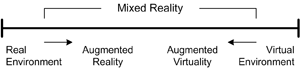
\includegraphics{./images/Milgram_Continuum}
\caption{\label{fig:milgram_continuum} Mixed Reality}
\end{center}
\end{figure}

Dalam \textit{augmented reality}, yang lebih dekat ke sisi kiri, lingkungan bersifat nyata dan benda bersifat maya, sementara dalam \textit{augmented virtuality}, yang lebih dekat ke sisi kanan, lingkungan bersifat maya dan benda bersifat nyata. 

\section{\textit{Komponen \textit{Augmented Reality}}}
\label{sec:komponen_ar}

\section{Teknik Display \textit{Augmented Reality}}
\label{sec:AR_display}
Sistem \textit{display} AR merupakan sistem manipulasi citra yang menggunakan seperangkat optik, elektronik, dan komponen mekanik untuk membentuk citra dalam jalur optik antara mata pengamat dan objek fisik yang akan digabungkan dengan teknik AR. Bergantung kepada optik yang digunakan, citra bisa dibentuk pada sebuah benda datar atau suatu bentuk permukaan yang kompleks (tidak datar)\cite{Bimber2005}. Gambar \ref{fig:diagram_display_AR} mengilustrasikan kemungkinan citra akan dibentuk untuk mendukung AR, peletakan display bergantung dari pandangan pengguna dan objek, dan tipe citra seperti apa yang akan dihasilkan (\textit{planar} atau \textit{curved}).

\begin{figure}[h]
	\begin{center}
	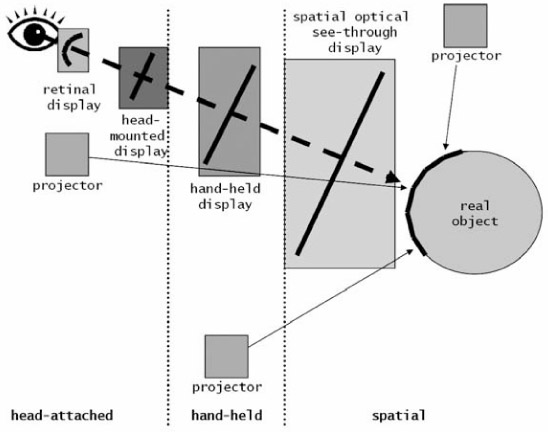
\includegraphics[width=10cm]{images/diagram_display_AR}
	\caption{\label{fig:diagram_display_AR}Pembentukan citra untuk display \textit{augmented reality}}
	\end{center}
\end{figure}

Secara garis besarnya ada tiga teknik display AR \cite{Bimber2005}, yaitu sebagai berikut:

\begin{enumerate}
\item \textit{Head-Attached Display}
\item \textit{Handheld Display}
\item \textit{Spatial Display}
\end{enumerate}

\subsection {\textit{Head-Attached Display}}
\label{subsec:HAD}
\textit{Head-Attached Display} merupakan teknik display yang mengharuskan penggunanya untuk memakai sistem ini di kepala pengguna. Berdasarkan teknik citra yang terbentuk, \textit{Head-Attached Display} terbagi tiga, yaitu sebagai berikut: 
\begin{itemize}
\item \textit{Head-Mounted Display}. 
\item \textit{Head-Mounted Projectors}.
\item \textit{Virtual Retina Display}. 
\end{itemize}
Kelebihan teknik display \textit{Head-Attached Display} ini adalah lebih nyaman ke pengguna, karena citra yang terbentuk mengikuti sudut pandang pengguna.

\subsubsection {\textit{Head-Mounted Display}}
\label{subsubsec:HMD}
\textit{Head-Mounted Display} (HMD) menggabungkan citra dari objek virtual dan objek nyata dan menampilkannya langsung ke mata pengguna melalui suatu alat yang dipasang di kepala pengguna. Terdapat dua tipe utama perangkat HMD yang digunakan dalam aplikasi realitas tertambah, yaitu \textit{optical-see-through} HMD dan \textit{video see-through} HMD. Keduanya digunakan untuk berbagai jenis pekerjaan dan memiliki keuntungan dan kerugian masing-masing. Dengan \textit{optical-see-through} HMD, lingkungan nyata dilihat melalui cermin semi transparan yang diletakkan di depan mata pengguna. Cermin tersebut juga digunakan untuk merefleksikan citra yang dibentuk oleh komputer ke mata pengguna, menggabungkan lingkungan nyata dan virtual. Dengan \textit{video see-through} HMD, lingkungan nyata direkam mengunakan dua kamera video yang terintegrasi ke alat, seperti gambar \ref{fig:actual_see_trough_HMD}, dan citra yang dibentuk komputer digabung dengan video tadi untuk merepresentasikan lingkungan yang akan dilihat pengguna \cite{Rolland1994}.

\begin{itemize}
\item {\textit{Video-see-through Head-Mounted Display}}

\begin{figure}[h]
\begin{center}
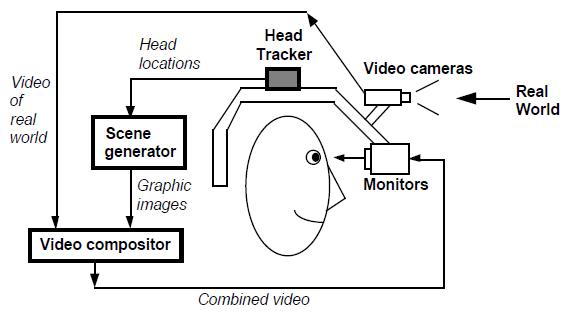
\includegraphics[width=11cm]{./images/opaque_HMD}
\caption{\label{fig:opaque_HMD} Diagram \textit{Opaque} HMD}
\end{center}
\end{figure}

\textit{Video see-through} HMD bekerja dengan menggabungkan sebuah \textit{closed-view} HMD dengan satu atau dua \textsl{head-mounted} kamera video, melalui kamera video tersebut pengguna melihat ke lingkungan nyata. Video dari kamera dikombinasikan dengan citra yang dibuat oleh \textit{scene generator}, dunia nyata dan virtual digabungkan. Hasilnya dikirimkan ke monitor yang terletak di depan mata pengguna. Gambar \ref{fig:opaque_HMD} menunjukkan konsep dari \textit{Video see-through} HMD, gambar \ref{fig:actual_opaque_HMD} adalah contoh \textit{Video see-through} HMD, dengan dua video terintegrasi di bagian atas Helm \cite{Azuma1997}.

\begin{figure}[h]
\begin{center}
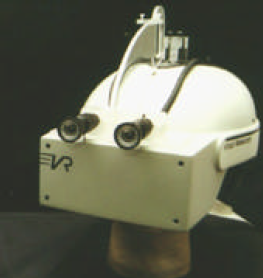
\includegraphics[width=5cm]{./images/actual_opaque_HMD}
\caption {\label{fig:actual_opaque_HMD} Contoh \textit{Opaque} HMD}
\end{center}
\end{figure}

\item {\textit{Optical see-through Head-Mounted Display}}

Tidak seperti penggunaan \textit{video see-through} HMD, \textit{optical see-through} HMD  menyerap cahaya dari lingkungan luar, sehingga memungkinkan pengguna untuk secara langsung mengamati dunia nyata dengan mata (gambar \ref{fig:see-trough_HMD}). Selain itu, sebuah sistem cermin yang diletakkan di depan mata pengguna memantulkan cahaya dari pencitraan grafis yang dihasilkan komputer. Pencitraan yang dihasilkan merupakan gabungan optis dari pandangan atas dunia nyata dengan pencitraan grafis \cite{Azuma1997}.

\begin{figure}[h]
\begin{center}
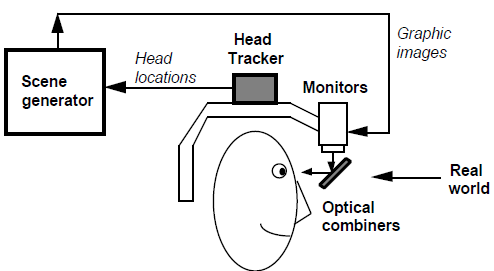
\includegraphics[width=11cm]{./images/see-trough_HMD}
\caption{\label{fig:see-trough_HMD} Diagram \textit{see-trough} HMD}
\end{center}
\end{figure}

\begin{figure}[h]
\begin{center}
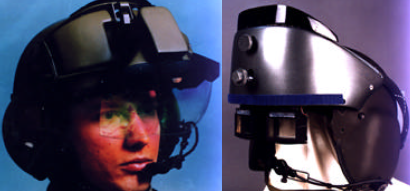
\includegraphics[width=10cm]{./images/actual_see-trough_HMD}
\caption {\label{fig:actual_see_trough_HMD} Contoh \textit{see-through} HMD, dibuat oleh Hughes Electronics}
\end{center}
\end{figure}

\end{itemize}

\subsubsection {\textit{Head-Mounted Projectors}}
\label{subsubsec:HMDP}
\textit{Head-Mounted Projectors} Menggunakan proyektor atau panel LCD kecil dan mempunyai cahaya sendiri untuk menampilkan citra langsung ke lingkungan nyata \cite{Bimber2005}. Seperti yang ditunjukkan oleh gambar \ref{fig:hmpd}.

\begin{figure}[h]
\begin{center}
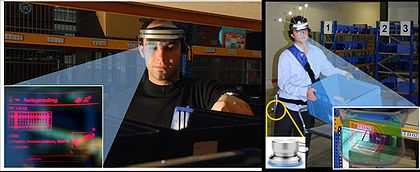
\includegraphics{./images/hmpd}
\caption {\label{fig:hmpd} Ilustrasi penggunaan dua jenis perangkat HMD yang digunakan untuk menampilkan data dan informasi tambahan}
\end{center}
\end{figure}

\subsubsection {\textit{Virtual Retina Display}}
\label{subsubsec:VRD}
\textit{Virtual retina display} (VRD), atau disebut juga dengan \textit{retinal scanning display} (RSD), memproyeksikan cahaya langsung kepada retina mata pengguna\cite{Haller2010}. VRD dapat menampilkan proyeksi citra yang penuh dan juga tembus pandang tergantung pada intensitas cahaya yang dikeluarkan, sehingga pengguna dapat menggabungkan realitas nyata dengan citra yang diproyeksikan  melalui sistem penglihatannya. VRD dapat menampilkan jarak pandang yang lebih luas daripada HMD dengan citra beresolusi tinggi\cite{Jacko2010}.  Keuntungan lain VRD adalah konstruksinya yang kecil dan ringan. Namun, VRD yang ada kini masih merupakan prototipe  yang masih terdapat dalam tahap perkembangan, sehingga masih belum dapat menggantikan HMD yang masih dominan digunakan dalam bidang AR. Gambaran sederhana VRD ini dapat dilihat pada gambar \ref{fig:VRD_diagram}.

\begin{figure}[h!]
	\centering
		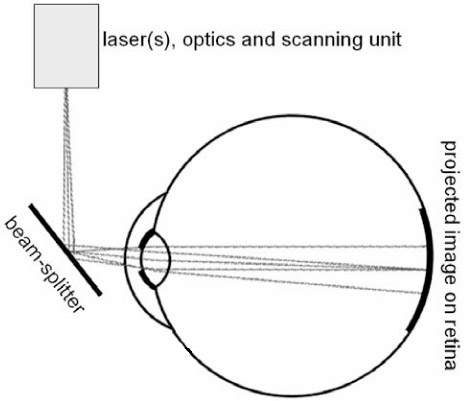
\includegraphics[width=6cm]{images/virtual_retina_diagram}
	\caption{\label{fig:VRD_diagram} Diagram sederhana \textit{virtual retina display}}
\end{figure}

%\begin{figure}[h]
%\begin{center}
%\includegraphics{./images/Vrd_blocks.gif}
%\caption{\label{fig:vrd_block} Diagram Blok \textit{Virtual Retina Display}}
%\end{center}
%\end{figure}

\subsection {\textit{Handheld Display}}
\label{subsec:handheld_display}
Teknik ini menggunakan alat dengan display yang dengan mudah dapat digenggam pengguna (Tablet PC, PDA dan telepon genggam) seperti yang ditunjukkan pada gambar \ref{fig:AR_phone}. Sensor dapat berupa GPS, kompas digital ataupun kamera yang ada pada \textit{handheld} tersebut. Semua penerapan AR pada perangkat genggam menggunakan kamera untuk menggabungkan citra digital dengan lingkungan nyata, \textit{Handheld} AR sangat menjanjikan untuk tujuan komersial. Dua kelebihan utama dari \textit{Handheld} AR adalah mobilitas perangkat yang mudah dan salah satu perangkat genggam yang banyak digunakan (telepon genggam) telah banyak dilengkapi kamera.

\begin{figure}[h!]
	\centering
		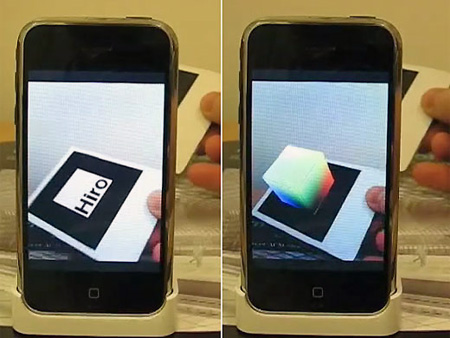
\includegraphics[width=8cm]{images/handphone_AR}
	\caption{\label{fig:AR_phone} Contoh augmented reality dengan \textit{handphone}}
\end{figure}

\subsection {\textit{Spatial Display}}
\label{subsec:spatial_display}
Dalam \textit{Spatial Augmented Reality} (SAR), objek nyata digabungkan langsung dengan citra yang terintegrasi langsung ke lingkungan nyata. Contohnya, citra diproyeksikan ke lingkungan nyata menggunakan proyektor digital atau tergabung dengan lingkungan menggunakan panel display \cite{Ramesh1998}. Perbedaan utama pada SAR dibanding teknik display sebelumnya adalah displaynya terpisah dengan pengguna. SAR memiliki kelebihan dari HMD dan handheld, sistem ini bisa digunakan oleh banyak orang pada waktu bersamaan tanpa perlu mengenakan suatu alat.

Ada tiga teknik display dalam SAR \cite{Bimber2005}, yaitu sebagai berikut:
\begin{enumerate}
\item \textit{Screen-Based Video See-Through Displays}\\
\textit{Screen-based }AR menggabungkan citra dan lingkungan nyata yang ditampilkan ke sebuah monitor, seperti yang ditunjukkan pada gambar \ref{fig:SAR_screen}.

\begin{figure}[h]
	\centering
		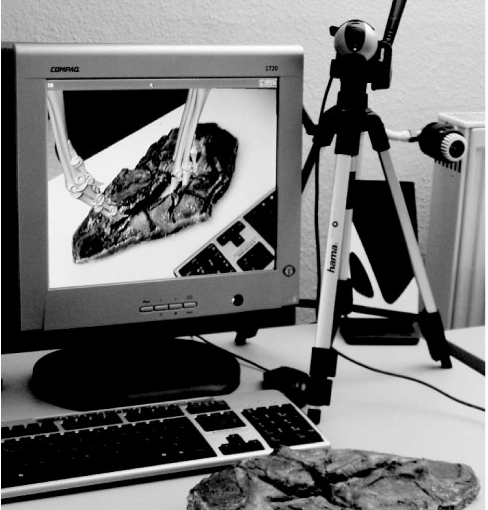
\includegraphics[width=6cm]{images/screen_SAR}
	\caption{\label{fig:SAR_screen} Contoh \textit{Screen-Based Video See-Through Displays} }
\end{figure}

\item \textit{Spatial Optical See-Through Displays}\\
Sistem ini menghasilkan citra yang ditampilkan langsung ke lingkungan nyata. Komponen yang penting dalam sistem ini meliputi \textit{spatial optical combiners} (\textit{planar} atau \textit{curved beam combiners}), layar transparan atau hologram.

\item \textit{Projection-Based Spatial Displays}\\
Sistem ini memproyeksikan citra secara langsung pada permukaan objek fisik daripada menampilkannya pada sebuah bidang pencitraan dalam penglihatan pengguna. Sistem ini menggunakan banyak proyektor yang digunakan untuk meningkatkan wilayah tampilan serta meningkatkan kualitas citra.

\end{enumerate}

\section{Model Tiga Dimensi (3D)}
\label{sec:model_3d}
Pemodelan Tiga Dimensi (3D) (3D \textit{modeling} atau dikenal juga dengan \textit{meshing}) adalah proses pembuatan representasi matematis permukaan tiga dimensi dari suatu objek dengan \textit{software} tertentu. Produk hasil pemodelan itu disebut model 3D. Model 3D tersebut dapat ditampilkan sebagai citra dua dimensi melalui sebuah proses yang disebut \textit{3D rendering}.
%
%Models may be created automatically or manually. The manual modeling process of preparing geometric data for 3D computer graphics is similar to plastic arts such as sculpting.
%
Model 3D direpresentasikan dari kumpulan titik dalam 3D, terhubung oleh berbagai macam entitas geometri, seperti segitiga, garis, permukaan lengkung, dan lain sebagainya. Berdasarkan hal tersebut, model 3D bisa dibuat manual (seperti seni memahat), secara algoritma (pemodelan prosedural), atau \textit{scanning}. Hasil akhir dari citra 3D adalah sekumpulan poligon. Model dengan jumlah poligon yang lebih banyak memerlukan waktu yang lebih lama untuk di-\textit{render} oleh komputer, karena setiap permukaan memiliki tekstur dan \textit{shading} tersendiri. 

\section{Aplikasi Komputer Berbasis Web (\textit{Rich Internet Application})}
\label{sec:aplikasi_web}

Pada tahun 90-an, "mengakses \textit{web}" berarti mengakses tulisan dan gambar statis secara \textit{online} . Sejalan dengan berkembangnya koneksi internet, kebutuhan akan suatu konten yang lebih kaya, responsif juga meningkat. Pada tahun 2002, Macromedia menemukan istilah \textit{Rich Internet applications} (RIAs). RIAs menggabungkan fleksibilitas, tingkat responsif, dan kemudahan aplikasi berbasis desktop. RIAs atau dikenal dengan aplikasi berbasis \textit{web} adalah aplikasi yang mempunyai karakteristik seperti aplikasi \textit{desktop}, biasanya didistribusikan atau diakses lewat \textit{browser web} standar, menggunakan \textit{web plug-in}. Contoh RIAs meliputi Ajax, Curl, GWT, Adobe Flash/Adobe Flex/AIR, Java/JavaFX, Mozilla's XUL dan Microsoft Silverlight. 

Aplikasi berbasis \textit{web} semakin banyak dikembangkan, karena kelebihan aplikasi \textit{web} yang sangat baik untuk aplikasi dengan model \textit{client-server}. Beberapa kelebihan aplikasi \textit{web} dibanding aplikasi \textit{desktop}:
\begin{enumerate}
	\item \textit{Running anywhere} (berjalan/beroperasi dimana saja), cukup instalasi pada satu \textit{server} dan tanpa perlu instalasi apapun selama ada \textit{web browser} di sisi \textit{client}, pengguna langsung  dapat menjalankan aplikasi tersebut tanpa konfigurasi apapun. Secara default, \textit{web browser} pada sistem operasi apapun telah tersedia sehingga kebutuhan akan \textit{web browser} untuk menjalankan aplikasi bukanlah suatu kendala berarti.
	\item \textit{Easy to update} (mudah untuk diubah/diperbaharui), cukup \textit{update} pada sisi \textit{server} maka aplikasi pada \textit{client} akan langsung menggunakan versi ter-\textit{update} tanpa harus instalasi dulu pada \textit{client}.
	\item \textit{Requirement} (kebutuhan)pada \textit{client} tidak terlalu besar. Karena \textit{running} aplikasi bersifat \textit{stateless} dan pada sisi \textit{client} hanya sebagai \textit{interface} maka spesifikasi hardware pada \textit{client} tidak harus canggih. 
	\item Tampilan yang lebih beragam.
\end{enumerate} 

\section {Adobe Flash \textit{Platform}}
\label{subsec:adobe_flash_platform}
Kebanyakan \textit{designer} dan \textit{developer} menggunakan Adobe Flash ataupun Adobe Flex, yang merupakan bagian dari platform Adobe Flash, untuk mengembangkan RIAs. Flash merupakan suatu \textit{environment} untuk membuat konten yang interaktif dan kaya fitur dalam dunia \textit{web}. Begitu juga Flex merupakan sebuah \textit{framework} \textit{cross-platform} untuk mengembangkan RIAs. Konten yang dibuat dengan Flash dan Flex di-\textit{deploy} menggunakan Adobe Flash Player

\subsection {Adobe Flash}
\label{subsec:adobe_flash}
Adobe Flash (dulunya Macromedia Flash) adalah platform multimedia yang aslinya dibuat oleh Macromedia dan saat ini dikembangkan dan didistribusikan oleh Adobe Systems. Sejak pengenalannya pada Tahun 1996, Flash telah menjadi metode yang popular untuk menambahkan animasi dan interaktivitas ke halaman web. Komponen Flash untuk mengintegrasikan video ke halaman web, dan yang terbaru saat ini, untuk mengembangkan RIAs.

Flash dapat memanipulasi vector dan raster grafik, serta mendukung \textit{streaming} dua arah audio dan video. Flash menggunakan bahasa \textit{script} yang disebut Action Script. Banyak produk \textit{software}, sistem dan \textit{device} dapat menampilkan konten flash, contohnya Adobe Flash player, yang tersedia gratis bagi sebagian besar \textit{web browser}. Beberapa ponsel dan alat elektronik lainnya juga dapat menampilkan konten Flash, menggunakan Flash lite.

\textit{File} dalam format SWF, biasanya disebut "ShockWave Flash movies", "Flash movies" atau "Flash games", yang biasanya memiliki sebuah ekstensi .swf dan dapat menjadi objek di halaman \textit{web}. \textit{File} tersebut pada dasarnya dijalankan dengan Flash Player itu sendiri atau digabungkan dengan "Projector" (\textit{video flash} yang dapat berjalan sendiri dengan ekstensi .exe di Microsoft Windows atau .hqx untuk Macintosh). \textit{File} Flash Video memiliki ekstensi .flv dan juga digunakan dalam .swf atau dijalankan melalui aplikasi yang dapat menjalankan \textit{file} flv.

\subsection {Adobe Flex}
\label{subsec:adobe_flex}
Adobe Flex adalah paket pengembangan \textit{software} yang dirilis oleh Adobe systems untuk pengembangan dan aplikasi \textit{cross-platform rich internet} berbasis platform adobe flash. Aplikasi flex dapat ditulis menggunakan Adobe Flash Builder sebagai IDE (\textit{Integrated Development Evironment}) dan menggunakan Flex \textit{Software Development Kit} (SDK) yang tersedia gratis dari Adobe. 

Flex membuat \textit{workflow} dan model pemrograman yang familiar terhadap \textit{developer} aplikasi berbasis \textit{web}. FLex menggunakan MXML dan ActionScript. MXML merupakan sebuah bahasa yang berbasis XML, menawarkan cara membangun dan menata \textit{user interface}. Interaktivitas dicapai melalui penggunaan ActionScript, yaitu bahasa utama Flash Player.

Flex menyediakan dua kompiler: mxmlc dan compc. Kompiler compc dan mxmlc bisa dijalankan dari Flex Builder atau pun dari \textit{command line}. compc digunakan untuk mengkompilasi komponen, kelas, and file lainnya ke file SWC atau RSL yang digunakan sebagai \textit{library} untuk aplikasi. mxmlc untuk mengkompilasi ActionScript dan SWC ke \textit{file} SWF, seperti ditunjukkan pada gambar \ref{fig:compile_flex}. Setelah aplikasi dikompilasi dan di-\textit{deploy} ke \textit{web server}, pengguna bisa mengakses file SWF tersebut dan dijalankan via \textit{web browser}.

\begin{figure}
\begin{center}
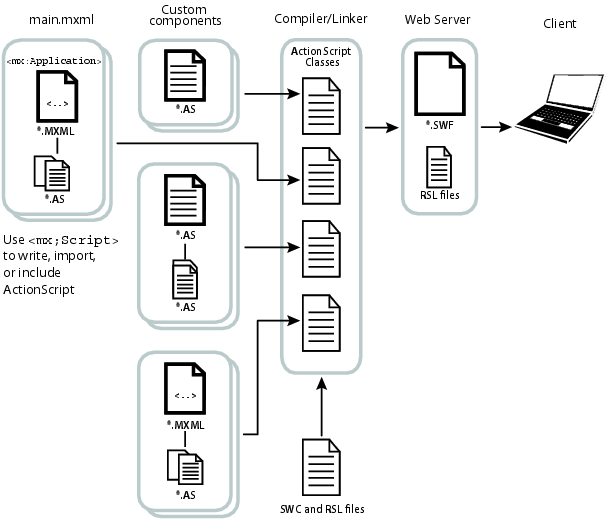
\includegraphics[width=9cm]{./images/compile_flex.png}
\caption{\label{fig:compile_flex} Diagram Kompilasi Flex}
\end{center}
\end{figure}

\subsection {ActionScript}
\label{subsec:action_script}
ActionScript merupakan bahasa pemrograman berorientasi objek yang berdasarkan ECMAScript (bahasa yang distandarisasi oleh Ecma International dalam spesifikasi ECMA-262 dan ISO/IEC 16262). ActionScript  terutama digunakan untuk pengembangan \textit{website} dan \textit{software} menggunakan Adobe Flash Player (dalam bentuk \textit{file} SWF yang diintegrasikan  ke halaman \textit{web}), ActionScript juga digunakan pada beberapa aplikasi untuk \textit{database}  (seperti Alpha Five). ActionScript pada awalnya didesain untuk mengatur animasi vektor 2D sederhana yang dibuat di Adobe Flash, dengan berkembangnya. Versi terakhir dari ActionScript menambahkan kemungkinan penggunaan  untuk pembuatan \textit{web} berbasis \textit{game} dan RIAs dengan media \textit{streaming} (seperti video dan audio).

\section{\textit{Library} Pendukung Augmented Reality Pada Platform Flash}
\label {sec:library_AR}
\textit{Library} atau Pustaka, dalam ilmu komputer adalah koleksi dari rutin-rutin program yang digunakan untuk membangun dan mengembangkan \textit{software}. \textit{Library}, umumnya mengandung kode program dan data pembantu (banyak \textit{programmer} menyebutnya sebagai \textit{helper}), yang menyediakan layanan-layanan kepada program-program independen. Penggunaan \textit{library} sangat diperlukan untuk mengembangkan aplikasi AR secara cepat. \textit{Library} AR yang dikenal luas dalam platform Flash adalah FLARToolKit.

\subsection {FLARToolKit}
\label {subsec:FLARToolKit}
%\subsection {FLARToolKit}
%\label{subsec:FLARToolKit}
%Pada bulan november 2008, sebuah grup pemrograman di Jepang, mengembangkan banyak proyek dengan ActionScript sehingga memberi ide kepada para \textit{developer} akan apa yang bisa dilakukan bahasa tersebut. FLARToolKit, pertama kali dikembangkan oleh Tomohiko Koyama (aka Saqoosha), ia mengenalkan AR ke dunia \textit{web}, dan ke segmen pengguna yang lebih luas.

FLARToolKit adalah \textit{tracking system library} yang bersifat \textit{open-source} sehingga memungkinkan \textit{programmer} dengan mudah mengembangkan aplikasi AR, FLARToolKit merupakan \textit{porting} (perubahan terhadap \textit{software} untuk menjadikannya dapat digunakan di lingkungan yang berbeda) yang paling terakhir dari ARToolkit, yaitu sebuah libary AR C++ yang awalnya dikembangkan oleh Dr. Hirokazu Kato di  Human Interface Technology Lab University of Washington. Dengan datangnya ActionScript 3.0, para pengembang seperti Mario Klingemann dan lainnya mulai bereksperimen dengan teknik analisis image secara \textit{real-time} untuk  Flash Player. Saqoosha meneruskan hal ini, dan mem-\textit{porting} FLARToolKit dari NYARToolkit (sebuah Java/C-sharp/Android \textit{port} dari ARToolkit).

FLARToolKit hanya merupakan \textit{library} untuk \textit{tracking} pada AR, untuk menampilkan objek 3D di lingkungan Flash, FLARToolKit memerlukan sebuah \textit{library} 3D. Beberapa \textit{library} 3D yang didukung oleh FLARToolKit adalah sebagai berikut:
\begin{itemize}
\item Alternativa3D
\item Away3D
\item Away3D Lite
\item Papervision3D
\item Sandy3D
\end{itemize}

Proses FLARToolKit secara garis besarnya sebagai berikut: 

\begin{enumerate}
	\item Mengambil video dari \textit{webcam}.
	\item Binarisasi citra masukan(\textit{thresholding}).
	\item Memberi penanda (\textit{labelling}).
	\item Deteksi area persegi (\textit{Marker Outline Detection}). 
	\item Pencocokan pola.
	\item Menghitung transform matrix.
	\item Merender obyek 3D.
\end{enumerate}

\subsubsection {Mengambil Video dari \textit{Webcam}}
\label{subsubsec:capture_webcam}
Langkah awal yang harus dilakukan adalah mendapatkan masukan video dari sebuah \textit{webcam}, seperti yang ditunjukkan gambar \ref{fig:capture_from_webcam}. Video yang di-\textit{streaming} secara \textit{real-time} ini akan diolah oleh sistem untuk dianalisa \textit{frame} per \textit{frame}. Sebelum \textit{webcam} digunakan, \textit{webcam} harus dikaliberasi terlebih dahulu. Kaliberasi \textit{webcam} merupakan bagian yang sangat penting dalam proses pengambilan masukan video. Hal ini disebabkan oleh distorsi pada lensa \textit{webcam} yang tiap-tiap kamera berbeda karakteristiknya (gambar \ref{fig:distorted_image}). Tujuan dari kalibrasi \textit{webcam} adalah untuk menghitung tingkat distorsi dari sebuah lensa \textit{webcam} yang digunakan agar citra yang dihasilkan mendekati citra ideal.

\begin{figure}[h]
\begin{center}
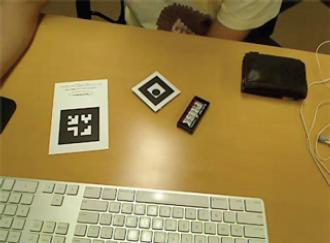
\includegraphics[width=7cm]{./images/flartk/capture_webcam.JPG}
\caption{\label{fig:capture_from_webcam} Mengambil citra dari \textit{webcam}}
\end{center}
\end{figure}

%Menggunakan \textit{class} kamera dan video kemudian menggambar video contohnya ke BitmapData. 

\begin{figure}[h]
\begin{center}
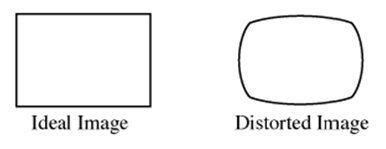
\includegraphics[width=6cm]{./images/flartk/distorted_image.JPG}
\caption{\label{fig:distorted_image} Perbandingan antara citra yang ideal dengan citra yang disebabkan oleh faktor distorsi}
\end{center}
\end{figure}

\subsubsection {Binarisasi Citra Masukan (\textit{Thresholding})}
\label{subsubsec:thresholding}
Langkah pertama pada aplikasi visi komputer yang terletak pada deteksi tepi adalah untuk men-\textit{threshold} sumber citra atau disebut juga binarisasi seperti yang ditunjukkan gambar \ref{fig:thresholding}. \textit{Thresholding} mengkonversi citra ke citra binari sehingga memudahkan untuk komputasi. Sebuah citra binari dibuat dengan mengubah pixel yang lebih cerah daripada nilai \textit{threshold} ke suatu warna, dan pixel yang lebih gelap daripada nilai \textit{threshold} ke suatu warna lainnya (didefinisikan sebagai \textit{gray-scale} atau hitam-putih). Nilai \textit{threshold} berada pada angka 0 – 255 dan secara default, \textit{threshold} bernilai 100. Fungsi dari proses ini adalah untuk membantu sistem agar dapat mengenali bentuk segi empat dan pola di marker pada citra yang diterima. Nilai \textit{threshold} dapat dirubah dan disesuaikan dengan kondisi cahaya disekitar \textit{marker} untuk tetap membuat \textit{marker} terlihat sebagai segi empat, karena ketika cahaya disekitar \textit{marker} berkurang ataupun berlebih pada saat proses \textit{thresholding}, sistem tidak dapat mendeteksi \textit{marker}.
%\begin{figure}[h]
%\begin{center}
%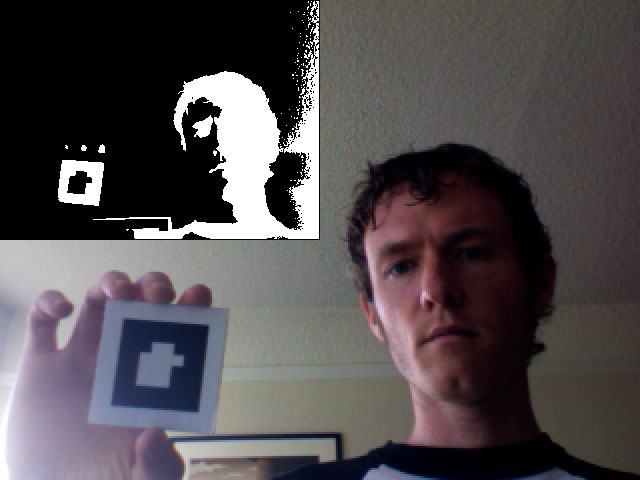
\includegraphics[width=7cm]{./images/thresholding}
%\caption{\label{fig:thresholding} Thresholding}
%\end{center}
%\end{figure}
\begin{figure}
\begin{center}
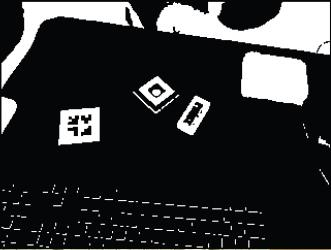
\includegraphics[width=7cm]{./images/flartk/binarize.JPG}
\caption{\label{fig:thresholding} Thresholding}
\end{center}
\end{figure}

\subsubsection {Memberi Penanda (\textit{Labeling})}
\label{subsubsec:labeling}
Langkah berikutnya dari FLARToolKit adalah menemukan area yang berdampingan dalam citra yang di-\textit{treshold}, khususnya dalam area dibawah \textit{threshold} (area yang lebih gelap). Area yang berdampingan diberi tanda dengan warna yang berbeda dengan tujuan untuk mengidentifikasi area, proses \textit{labelling} dapat dilihat pada gambar \ref{fig:labelling}.
%Dengan menggunakan fungsi \textit{BitmapData.getColorBoundsRect} dan \textit{BitmapData.foodFill}, 

\begin{figure}[h]
\begin{center}
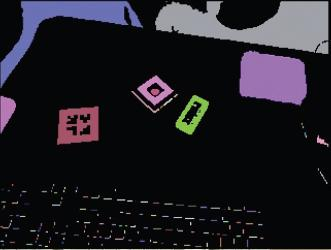
\includegraphics[width=7cm]{./images/flartk/labelling.JPG}
\caption{\label{fig:labelling} Setiap area putih ditandai dengan warna yang berbeda.}
\end{center}
\end{figure}

\subsubsection {Deteksi Area Persegi (\textit{Marker Outline Detection})}
\label{subsubsec:outline_detection}
Langkah selanjutnya, FLARToolKit mencari area yang kemudian ditandai sebagai persegi \textit{(marker outline)}. Setelah citra mengalami proses \textit{thresholding} dan \textit{labelling}, FLARToolkit akan mengenali bentuk dan pola yang ada pada marker. FLARToolkit akan mencari bagian yang memiliki bentuk segi empat dan menandainya. FLARToolKit juga akan menghilangkan area yang tidak berbentuk segi empat sehingga yang akan ditampilkan pada layar hanyalah area yang memiliki bentuk segi empat (gambar \ref{fig:find_squares}.
%With candidates for marker locations, FLARToolKit then proceeds to search the labeled areas for shapes that could be transformed squares (i.e. marker outlines).

\begin{figure}[h]
\begin{center}
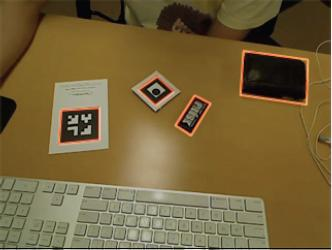
\includegraphics[width=7cm]{./images/flartk/find_squares.JPG}
\caption{\label{fig:find_squares} Mencari area persegi (Marker Outline Detection)}
\end{center}
\end{figure} 

\subsubsection {Pencocokan Pola}
\label{subsubsec:pattern_matching}
Setelah semua area persegi ditandai, FLARToolKit menganalisa citra yang berada di dalam persegi dan membandingkan polanya dengan sekumpulan pola yang telah ditentukan (pencocokan pola). FLARToolKit mengekstrak pola di dalam persegi menggunakan transformasi \textit{homography}. FLARToolKit memberikan sebuah nilai '\textit{confidence}' kepada setiap pola yang cocok, jika kecocokannya di atas nilai yang telah ditentukan maka polanya dinyatakan cocok. 

\begin{figure}
\begin{center}
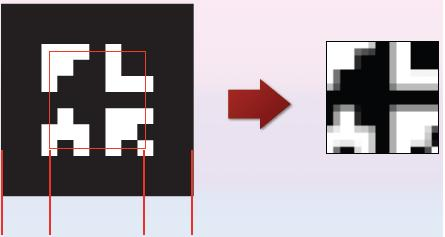
\includegraphics[width=7cm]{./images/flartk/marker_spec.JPG}
\caption{\label{fig:marker_spec} Spesifikasi pola marker}
\end{center}
\end{figure} 

Spesifikasi pola marker (gambar \ref{fig:marker_spec}):
\begin{itemize}
	\item Harus berupa persegi.
	\item Hanya 50\% dari tengah area yang digunakan untuk proses pencocokan pola.
	\item Pola marker secara \textit{default}-nya adalah 16 x 16 titik.
	\item Ukuran pola bisa lebih besar, tapi membutuhkan waktu yang lebih lama untuk diproses.
\end{itemize}

%\begin{figure}[h!]
%	\begin{center}
%		\subfloat {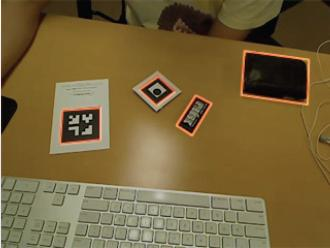
\includegraphics[width=5cm]{./images/flartk/matching_pattern.JPG} \label{fig:pattern_matching1}}\\
%		\subfloat {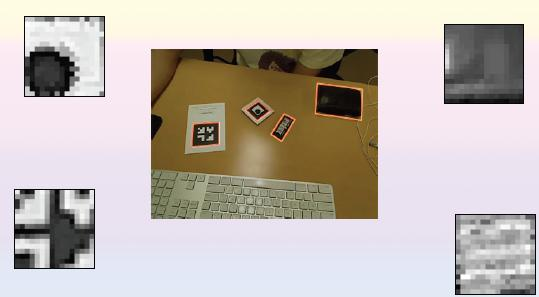
\includegraphics[width=5cm]{./images/flartk/matching_pattern2.JPG} \label{fig:pattern_matching2}}\\
%		\subfloat {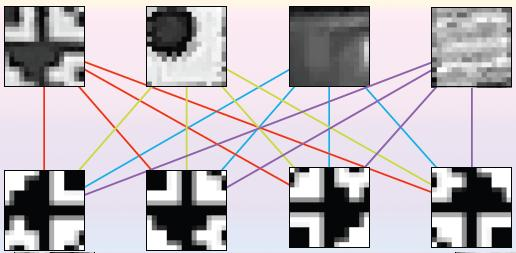
\includegraphics[width=5cm]{./images/flartk/matching_pattern3.JPG} \label{fig:pattern_matching3}}\\
%		\subfloat {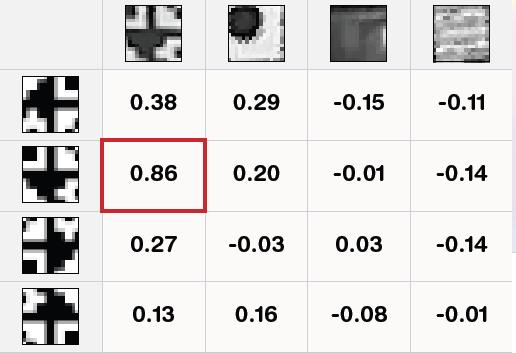
\includegraphics[width=5cm]{./images/flartk/matching_pattern4.JPG} \label{fig:pattern_matching4}}
%		\caption {\label{fig:pattern_matching} Proses pencocokan pola}
%	\end{center}
%\end{figure}

\subsubsection {Menghitung Transformasi Matriks}
\label{subsubsec:calculate_transform_matrix}
Transformasi matriks dihitung dari titik-titik persegi marker yang dideteksi. Matriks tersebut digunakan untuk proses \textit{render} objek 3D.% Algoritmanya dapat dilihat dalam paper di http://www.hitl.washington.edu/artoolkit/publications/.
%
%\begin{figure}[h!]
%\begin{center}
%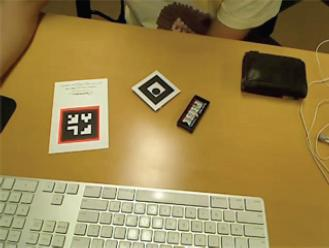
\includegraphics[width=7cm]{./images/flartk/calculate_transform_matrix.JPG}
%\caption{\label{fig:calculate_matrix} Kalkulasi transformasi matriks}
%\end{center}
%\end{figure} 

\subsubsection {Me-\textit{render} Objek 3D}
\label{subsubsec:render_the_3d_objects}
FLARToolKit menggunakan transformasi matriks yang dikalkulasikan di step sebelumnya dan menampilkan objek yang sesuai dengan sebuah \textit{library} 3D, seperti yang ditunjukkan gambar \ref{fig:render_3d_objects}. FLARToolKit menyertakan kelas pendukung yang mengkonversikan transformasi matriks FLARTollKit ke setiap kelas matriks internal \textit{library} 3D tersebut.

\begin{figure}[h!]
\begin{center}
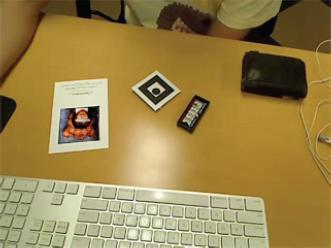
\includegraphics[width=7cm]{./images/flartk/render_3d_objects.JPG}
\caption{\label{fig:render_3d_objects} Render objek 3D}
\end{center}
\end{figure} 

\subsection {Papervision3D}
\label{subsec:Papervision3D}
Salah satu \textit{library} 3D (biasa disebut juga dengan \textit{engine} 3D) untuk platform Flash adalah Papervision3D, Papervison3D merupakan \textit{library} 3D yang bersifat \textit{open source}. Dengan Papervision 3D, model 3D bisa dibuat di platform Flash menggunakan kelas-kelas dalam ActionScript ataupun juga dengan meng-\textit{import} model yang dibuat dari \textit{software} pemodelan 3D. Model yang telah dibuat atau di-\textit{import}, bisa dikendalikan dengan ActionScript.

\subsection {FLARManager}
\label{subsec:FLARManager}
Visi komputer dalam konteks \textit{web} memiliki banyak kesulitan untuk diterapkan. Masalah utama ialah kurangnya kendali terhadap kondisi lingkungan \textit{end-user}. Kurangnya atau ketidakteraturan pencahayaan membuat analisis dari sebuah citra sangat sulit, dan permasalahan tersebut berdampak pada FLARToolKit. Selain itu, FLARToolKit sangat sulit digunakan karena minimnya dokumentasi, dan \textit{developer} harus membuat sebuah \textit{manager} untuk mengatur konfigurasi kamera, marker dan juga objek virtual yang akan ditampilkan. 

FLARManager adalah sebuah \textit{framework} sederhana yang memudahkan untuk membuat aplikasi AR dengan Flash terutama yang menggunakan \textit{libray} FLARToolKit. \textit{Framework} merupakan kumpulan komponen kelas sekaligus kerangka dalam pemrograman yang memudahkan \textit{programmer} untuk membuat suatu aplikasi yang siap pakai. FLARManager bisa meningkatkan akurasi dan reabilitas dari proses dengan hanya merubah konfigurasinya yang berupa file dengan format xml. FLARManager dapat mendeteksi lebih dari satu \textit{marker} dan pola dalam waktu bersamaan, sehingga bisa menampilkan objek virtual lebih dari satu.

FLARToolkit menyediakan akses ke sumber citra yang diprosesnya, dan juga hasil dari FLARToolkit setelah di analisa. Dengan demikian, FLARManager bisa difokuskan pada fungsionalitas dalam deteksi dan \textit{tracking} dari \textit{marker}. FLARManager sebisa mungkin menghindari perubahan terhadap FLARToolkit. Dengan tidak tergantungnya FLARManager terhadap FLARToolkit, setiap proyek bisa terus dikembangkan secara terpisah, dan FLARManager secara teori bisa diterapkan pada \textit{libray} Flash AR lainnya.

Sampai saat tulisan ini dibuat, FLARManager telah mendukung \textit{tracking library} sebagai berikut :
\begin{itemize}
\item FLARToolkit
\item flare*tracker
\item flare*NFT
\end{itemize}



%==========================================================================================================
% MULAI BAB III
%==========================================================================================================
\chapter{PERANCANGAN DAN IMPLEMENTASI}
\label{chap:perancangan}
%==========================================================================================================
% subbab
%==========================================================================================================
\section {Deskripsi}
\label{sec:gambaran_aplikasi}
Secara konvensional model suatu objek nyata (misalnya gedung) biasanya disajikan dengan membuat sebuah  miniatur atau maket seperti yang ditunjukkan gambar \ref{fig:real_virtual_ar}.a. Dengan adanya model atau maket tersebut, seseorang bisa dengan mudah melihat atau mengetahui objek yang dimodelkan tersebut secara nyata, akan tetapi pembuatan model atau maket tersebut membutuhkan waktu yang lama serta biaya yang mahal. Dengan menggunakan komputer dan \textit{software} tertentu pemodelan objek bisa disajikan secara virtual seperti terlihat pada gambar \ref{fig:real_virtual_ar}.b. Dengan menggunakan \textit{software}, pemodelan objek memang lebih menghemat biaya serta waktu, namun interaksi dengan dunia nyata sangat kurang. Aplikasi \textit{viewer} model 3D  dengan teknologi \textit{Augmented Reality} yang penulis rancang ini menggabungkan kedua kelebihan pemodelan secara nyata dan \textit{software}, yaitu kemudahan pembuatan model 3D (secara virtual) dan juga interaksi terhadap dunia nyata seperti diilustrasikan pada gambar \ref{fig:real_virtual_ar}.c.

\begin{figure}[h]
\begin{center}
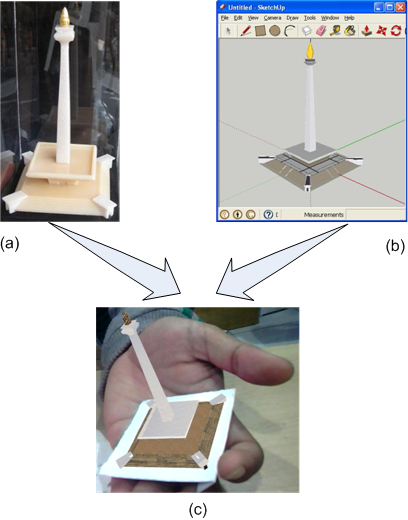
\includegraphics[width=10cm]{./images/real_virtual_ar}
\caption{\label{fig:real_virtual_ar} Gambaran aplikasi \textit{viewer} objek 3D virtual dengan \textit{Augmented Reality}}
\end{center}
\end{figure}

Aplikasi yang dirancang dengan teknologi AR ini, seolah-olah menggabungkan objek virtual dengan objek nyata, dalam hal ini objek nyatanya berupa gambar dengan pola tertentu (disebut \textit{marker}) dan objek virtualnya berupa model 3D. Sistem menggunakan teknik \textit{spatial display} (pembahasan pada subbab \ref{subsec:spatial_display} dengan \textit{screen display} (bisa berupa monitor ataupun proyektor). Secara garis besarnya gambaran sistem dapat dilihat pada gambar \ref{fig:gambaran_sistem_ar}. 
%Kamera yang terhubung ke komputer  menangkap sebuah citra dari \textit{marker} yang berfungsi sebagai \textit{tracker}. Dengan adanya pengenalan pola, sistem akan mengenali gambar tersebut. Setelah pola tersebut terindentifikasi maka sistem akan menampilkan model 3D yang telah ditentukan jika pola tersebut ditemukan. Proses tersebut berlangsung secara \textit{real-time} sehingga objek virtual yang tampil di komputer akan mengikuti pergerakan \textit{tracker}.
\begin{figure}[h]
\begin{center}
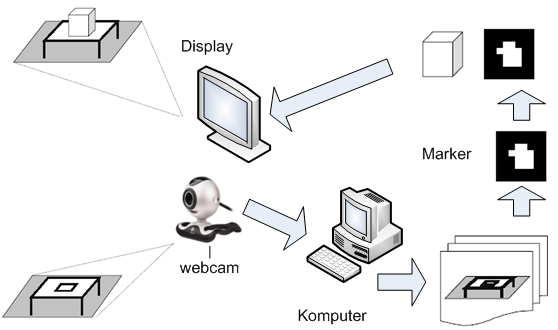
\includegraphics[width=10cm]{./images/gambaran_sistem_ar}
\caption{\label{fig:gambaran_sistem_ar} Gambaran sistem secara umum}
\end{center}
\end{figure}

\textit{webcam} berfungsi sebagai media \textit{visi} bagi aplikasi AR untuk mendapatkan video masukan. Kamera mengambil \textit{frame}-\textit{frame} video untuk dapat diterima oleh komputer. Komputer memproses citra digital yang diakuisisi oleh \textit{webcam}, \textit{frame} demi \textit{frame}. Komputer akan mendeteksi pola yang mirip dengan \textit{marker} dari setiap \textit{frame} video tersebut, yang kemudian lokasi dan rotasi dari \textit{marker} dapat ditentukan. Dengan informasi tersebut, objek \textit{virtual} digabungkan dengan video dari \textit{webcam} dan me-\textit{render}-nya sesuai dengan informasi posisi yang diperoleh dari \textit{marker} tersebut. Dengan demikian, \textit{marker} tersebut seolah-olah berfungsi sebagai \textit{tracker} untuk model 3D virtual. Proses tersebut berlangsung secara \textit{real-time} sehingga model 3D virtual yang tampil di media \textit{display} akan mengikuti pergerakan \textit{tracker}.

%FLARToolKit memiliki kelemahan dalam hal \textit{rendering} model. Sehingga sebuah \textit{library} yang dapat merender model 3D dengan kualitas tinggi seperti Papervison3D diperlukan. Papervision3D akan meload data objek 3D dan menampilkan objek tersebut. Pada aplikasi ini penulis menggunakan objek 3D dengan format collada yang sudah didukung oleh Papervision3D

\section {Perancangan Aplikasi}
\label{sec:desain_aplikasi}
Aplikasi yang dirancang merupakan aplikasi berbasis \textit{web} atau disebut juga \textit{Rich Internet Applications} (RIAs), tujuannya agar mudah diakses dari komputer atau juga \textit{handheld} tanpa perlu instalasi aplikasi. Berdasarkan penjelasan pada subbab \ref{subsec:adobe_flash_platform}, penulis memilih Adobe Flash sebagai \textit{Framework} RIAs dengan SDK (\textit{software Development Kit}) Adobe Flex. Bahasa script yang digunakan adalah ActionScript yang merupakan bahasa pemrograman berorientasi objek. ActionScript mendukung \textit{event-driven programming} (Pemrograman berbasis \textit{event}). \textit{event-driven programming} merupakan paradigma pemrogaman yang alur program ditentukan dari \textit{event}, \textit{input} sensor atau pesan dari program lain. Paradigma ini sangat cocok untuk pengembangan aplikasi ini, dikarenakan aplikasi menerima input dari kamera atau \textit{webcam}.

Aplikasi ini dibangun menggunakan FLARManager, seperti telah dijelaskan pada subbab \ref{subsec:FLARManager}, FLARManager dapat mempermudah dan mempercepat pengembangan aplikasi yang menggunakan \textit{library} FLARToolKit. \textit{Library} FLARToolKit merupakan salah satu \textit{tracking library} AR di lingkungan Flash (subbab \ref{subsec:FLARToolKit}). Di dalam FLARManager sudah termasuk pengaturan kamera untuk masukan video, kelas untuk mengatur pola marker yang digunakan, dan juga kelas untuk memudahkan interaksi dengan \textit{library} engine 3D, dengan demikian aplikasi yang dibangun tidak perlu berhubungan langsung dengan \textit{library} FLARToolKit.

\begin{figure}[h]
\begin{center}
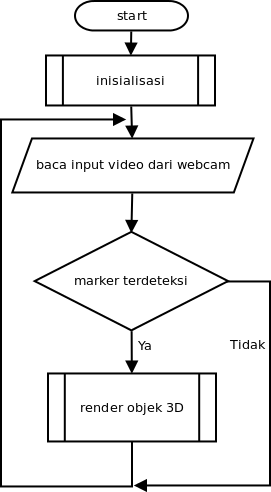
\includegraphics[width=6cm]{./images/flowchart/aplikasi}
\caption{\label{fig:flowchart_aplikasi} Diagram alir aplikasi secara umum}
\end{center}
\end{figure}

Secara keseluruhan, aplikasi dapat digambarkan dengan diagram alir pada gambar \ref{fig:flowchart_aplikasi}. Aplikasi melakukan inisialisasi terlebih dahulu sebelum melakukan \textit{tracking} \textit{marker}, \textit{marker} dideteksi dari masukan video \textit{webcam}, jika \textit{marker} terdeteksi maka objek 3D di-\textit{render}. 

Secara garis besarnya, dalam perancangan aplikasi ini ada tiga bagian utama yaitu sebagai berikut:
\nopagebreak
\begin{itemize}
\item Inisialisasi\\
Inisialisasi semua hal yang diperlukan untuk proses aplikasi (\textit{marker}, objek 3D, engine 3D)
\item \textit{Tracking} \textit{marker}\\
Marker yang digunakan lebih dari satu pola, setiap \textit{marker} dengan pola tertentu akan menjadi \textit{tracker} objek 3D tertentu pula.
\item \textit{Rendering} objek 3D\\
Objek 3D dirender dan diatur posisinya sesuai dengan posisi \textit{marker} yang terdeteksi.
\end{itemize}

Penulis merancang aplikasi ini atas beberapa kelas (gambar \ref{fig:diagram_kelas}), agar memudahkan pengembangan aplikasi. Kelas utama adalah \textbf{AR3DV}, yang mengatur jalannya aplikasi, mulai dari inisialisasi hingga \textit{render} objek 3D. 

\begin{figure}[h]
\begin{center}
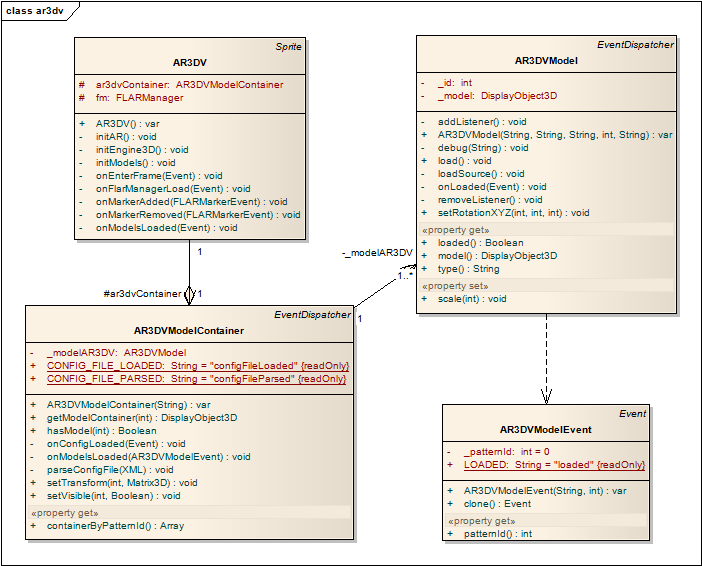
\includegraphics[width=14cm]{./images/class}
\caption{\label{fig:diagram_kelas} Diagram kelas aplikasi}
\end{center}
\end{figure}

Tiga kelas lainnya berhubungan dengan objek 3D dan inisialisasinya, yaitu sebagai berikut:
\begin{itemize}
\item AR3DVModelContainer\\
Kelas yang mengatur objek 3D apa saja yang di-\textit{load}, serta menyediakan objek 3D yang dapat dipanggil dari kelas utama. \textbf{AR3DVModelContainer} menggunakan file konfigurasi dengan format xml untuk model objek 3D yang akan di-\textit{load}.
\item AR3DModel\\
Kelas yang berfungsi untuk me-\textit{load} objek 3D, serta mengatur rotasi dan skala objek.
\item AR3DModelEvent\\
\textit{Loading} model memerlukan waktu yang cukup lama tergantung ukuran \textit{file} objek 3D. Karena itu \textit{load} objek 3D dilakukan secara asinkron. Kelas \textbf{AR3DVModelContainer} akan me-\textit{load} semua \textit{file} objek 3D dengan bantuan kelas \textbf{AR3DModel}. Agar kelas \textbf{AR3DVModelContainer} mengetahui objek 3D tertentu telah di-\textit{load}, diperlukan sebuah pesan yang disebut juga \textbf{Event}. Penulis membuat kelas \textbf{AR3DModelEvent} agar bisa digunakan \textbf{AR3DModel} untuk menyampaikan pesan ke kelas \textbf{AR3DModelContainer}.
\end{itemize}

\subsection{Inisialisasi}
\label{subsec:inisialisasi}
Pada tahap ini ditentukan \textit{marker} yang akan digunakan, sumber input video nya, objek 3D yang akan digunakan serta \textit{engine} 3D yang digunakan untuk me-\textit{render} objek 3D. Pada bagian inisialisasi ini, objek 3D diinisialisasi terlebih dahulu karena \textit{loading} objek 3D memerlukan waktu yang cukup lama. Setelah objek 3D di-\textit{load}, kemudian FLARManager dan \textit{engine} 3D diinisialisasi. Deskripsi inisialisasi digambarkan oleh \textit{sequence diagram} gambar \ref{fig:init_sequence}.

\begin{figure}[h]
\begin{center}
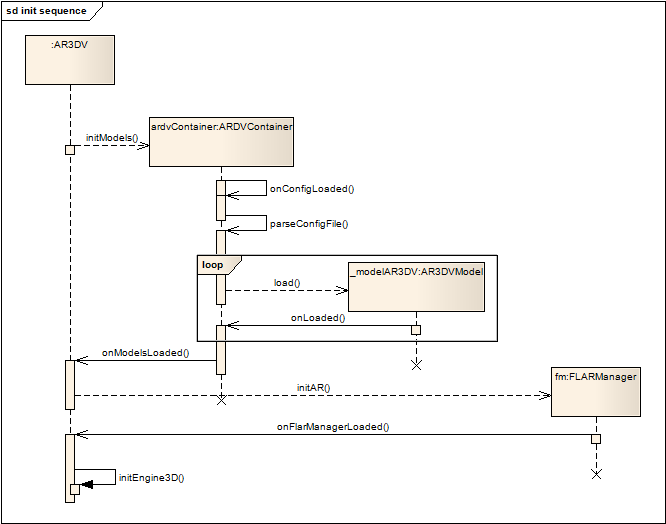
\includegraphics[width=14cm]{./images/init_sequence}
\caption{\label{fig:init_sequence} \textit{Sequence diagram} inisialisasi}
\end{center}
\end{figure}

\subsubsection {Inisialisasi Model 3D}
\label{subsubsec:inisialisasi_model_3d}
Model 3D yang akan ditampilkan di-\textit{load} terlebih dahulu. Agar aplikasi dapat menampilkan objek 3D tertentu tanpa merubah atau membangun ulang aplikasi, diperlukan sebuah \textit{file} konfigurasi untuk menentukan objek 3D yang akan di-\textit{load} sesuai dengan pola \textit{marker} yang dideteksi. File konfigurasi itu berisi informasi format file objek 3D yang digunakan, skala objek 3D dan juga rotasi terhadap koordinat xyz sehingga penampilan objek 3D bisa lebih proporsional. Dengan adanya file konfigurasi tersebut, objek 3D dan \textit{marker} yang digunakan dapat diatur dengan mudah.

Method untuk inisialisasi model 3D ini adalah \textbf{initModels}. Method ini akan membuat objek baru \textbf{AR3DVModelContainer}, yang akan me-\textit{load} objek-objek 3D sesuai konfigurasi file xml nya. Objek 3D di-\textit{load} satu persatu dengan bantuan \textbf{AR3DModel}, setelah semua objek ter-\textit{load}, sebuah pesan akan dikirim ke kelas utama (\textbf{AR3DV}) dan proses selanjutnya dapat dijalankan.

\subsubsection {Inisialisasi FLARManager}
\label{subsubsec:inisialisasi_flarmanager}
FLARManager merupakan inti dari aplikasi ini. FLARManager akan mengatur semua hal yang berkaitan dengan AR, mulai dari \textit{marker}, video masukan dari kamera, dan pengenalan \textit{marker} dengan bantuan \textit{library} FLARToolKit. FLARManager diinisialisasi dengan membuat objek baru FLARManager yang memerlukan file konfigurasi berupa file berformat xml dan objek \textit{tracker} (dalam hal ini FLARToolKit), kelas \textit{tracker} yang digunakan untuk objek \textit{tracker} adalah \textbf{FLARToolkitManager} yang juga telah tersedia dalam \textit{framework} FLARManager. Inisialisasi FLARManager terdapat pada method \textbf{initAR}, setelah FLARManager selesai di inisialisasi, method \textbf{onFlarManagerLoad} dijalankan.

\subsubsection {Inisialisasi \textit{Engine} 3D}
\label{subsubsec:inisialisasi_engine3d}
Untuk merender objek 3D, terutama objek 3D dari file, diperlukan \textit{library} pendukung atau disebut juga \textit{engine} 3D Flash. Penulis menggunakan Papervision3D (penjelasan mengenai Papervision3D dapat dilihat pada subbab \ref{subsec:Papervision3D}) sebagai \textit{library engine} 3D nya. Sebelum merender objek 3D, Papervision3D juga perlu diinisialisasi terlebih dahulu, inisialisasi engine 3D terdapat pada method \textbf{initEngine3D}.

\subsection{\textit{Tracking} Marker}
\label{subsec:tracking_marker}
Bagian ini merupakan inti dari AR, \textit{library} FLARToolKit bekerja pada bagian ini. Marker yang akan digunakan sebagai \textit{tracker} telah ditentukan pada bagian inisialisasi. Di dalam FLARManager telah terdapat kelas tersendiri yang menangani proses \textit{sampling} video, integrasi dengan FLARToolKit untuk pengenalan pola dan menentukan posisi \textit{marker}-nya. Ketika sebuah \textit{marker} terdeteksi, maka method yang mengatur \textit{tracking} \textit{marker} \textbf{onMarkerAdded} dan \textbf{onMarkerRemoved} dijalankan. Kedua method tersebut menentukan apa yang akan dilakukan aplikasi ketika \textit{marker} ditemukan. Jika \textit{marker} terbaca oleh sistem, method \textit{set} \textbf{visible} yang berfungsi untuk memunculkan objek 3D pada kelas AR3DModelContaner dijalankan. Begitu juga jika \textit{marker} tidak terbaca sistem method \textit{set} \textbf{visible} diisi nilai \textit{false} yang berarti objek 3D disembunyikan. %Gambaran proses pada saat \textit{marker} ditemukan dan tidak ditemukan lagi, bisa dilihat pada gambar sequence diagram \ref{fig:sequence_tracking_marker}.

\subsection{\textit{Rendering} objek 3D}
\label{subsec:render_objek3D}
Setelah \textit{marker} ditemukan maka, objek 3D di-\textit{render} atau dimunculkan diatas \textit{marker}, posisi dan rotasi objek 3D akan mengikuti \textit{tracker}. Method yang berkaitan dengan hal ini adalah \textbf{onEnterFrame}. Setiap objek dalam \textbf{AR3DModelContainer} akan diatur posisinya sesuai \textit{marker} yang berkaitan dengan objeknya.

\section {Implementasi Perancangan Aplikasi}
\label{sec:implementasi_perancangan_aplikasi}
Berdasarkan rancangan kelas dan \textit{sequence diagram}, kelas-kelas yang diperlukan dibangun. Penulis menggunakan Adobe Flash Builder sebagai \textit{Integrated Development Tools} (IDE) untuk mengembangkan aplikasinya. SDK yang digunakan adalah Flex versi 4.1. Dengan Adobe Flash Builder, proses \textit{debugging} dan \textit{deploy} aplikasi dapat mudah dilakukan.

Sesuai dengan rancangan pada subbab \ref{subsec:inisialisasi}, berikut ini adalah penjelasan mengenai \textit{source code} yang dibuat yang penulis bangun sesuai dengan rancangan. 

\subsection {Inisialisasi}
\label{subsec:implementasi_inisialisasi}
ActionScript telah menyediakan kelas \textbf{Sprite} untuk menampilkan semua objek yang akan digambarkan (\textit{drawing objects}). Kelas utama \textbf{AR3DV} dibangun dengan mewarisi kelas \textbf{Sprite} tersebut. Semua objek dan komponen lainnya ditambahkan ke kelas utama tersebut.

\subsubsection {Inisialisasi Model 3D}
\label{subsubsec:implementasi_inisialisasi_model3d}
Inisialisasi FLARManager terdapat pada method \textbf{initModels}, seperti ditunjukkan pada \textit{listing} \ref{init_model}.
\begin{lstlisting}[language=ActionScript,caption=Inisialisasi model,label=init_model]
private function initModels():void{
	// load model source dan konfigurasinya
	this.ar3dvContainer = new AR3DVModelContainer("../resources/ar3dv.xml");
	this.ar3dvContainer.addEventListener(AR3DVModelContainer.CONFIG_FILE_PARSED,this.onModelsLoaded);
}
\end{lstlisting}

Objek baru \textbf{AR3DVModelContainer} dibuat dan disimpan dalam variabel \textbf{ar3dvContainer}. \textbf{AR3DVModelContainer} memerlukan file konfigurasi (ar3dv.xml) yang berisi informasi lokasi file 3D, format file, rotasi xyz dan skala objek 3D (lampiran). Pertama kali dibentuk, objek \textbf{ar3dvContainer} akan meload file konfigurasi tersebut menggunakan \textbf{URLLoader}, seperti ditunjukkan \textit{listing} \ref{config-loader}.

\begin{lstlisting}[language=ActionScript,caption=Load Config AR3DV,label=config-loader]
public function AR3DVModelContainer(url:String){
	_configFileLoader = new URLLoader();
	_configFileLoader.addEventListener(IOErrorEvent.IO_ERROR, this.onConfigLoaded);
	_configFileLoader.addEventListener(SecurityErrorEvent.SECURITY_ERROR, this.onConfigLoaded);
	_configFileLoader.addEventListener(Event.COMPLETE, this.onConfigLoaded);
	_configFileLoader.load(new URLRequest(url));
}
\end{lstlisting}

Sebuah \textit{listener} ditambahkan ke objek \textbf{configLoader}, sehingga setelah file selesai di-\textit{load}, method \textbf{onConfigLoaded} dapat dijalankan dan file xml dapat diproses oleh method \textbf{parseConfigFile}, seperti yang ditunjukkan oleh listing \ref{parse-config}. 

\begin{lstlisting}[language=ActionScript,caption=Proses config file,label=parse-config]
private function parseConfigFile(data:XML):void{
	var modelList:XMLList = data.models;
	_containerByPatternId = new Array();
	_modelContainers = new Array();
	for each (var elem:XML in modelList.model) {
		this.debug("load model :"+elem.@name);
		var modelAR3DV:AR3DVModel = new AR3DVModel(elem.@name,elem.@source_dir,elem.@source,int(elem.@pattern),elem.@type);
		if(modelAR3DV.model!=null){
			modelAR3DV.addEventListener(AR3DVModelEvent.LOADED,this.onModelsLoaded);
			modelAR3DV.setRotationXYZ(int(elem.@x),int(elem.@y),int(elem.@z));
			modelAR3DV.scale = int(elem.@scale);
			modelAR3DV.load();
		}			
		_modelContainers[int(elem.@pattern)] = modelAR3DV;
	}
}
\end{lstlisting}

Method \textbf{parseConfigFile} akan me-\textit{load} objek 3D dengan bantuan objek \textbf{modelAR3DV} yang merupakan objek dari kelas AR3DVModel. Objek model disimpan dalam \textit{array} dengan \textit{key index}-nya berupa nomor pola \textit{marker} yang ditentukan di file konfigurasi model (ar3dv.xml).  

\subsubsection {Inisialisasi FLARManager}
\label{subsubsec:implementasi_inisialisasi_flarmanager}

Setelah model di-\textit{load}, maka method \textbf{initAR} pun dijalankan yang merupakan inisialisasi FLARManager. Seperti ditunjukkan pada potongan \textit{listing} method \textbf{initAR} \ref{code:init-fm}.

\begin{lstlisting}[language=ActionScript,caption=Init FLARManager,label=code:init-fm]
	/* Augmented reality initialisation */
	private function initAR():void {
		/* Initialise FLARManager */
		this.fm =  new FLARManager("../resources/flar/flarConfig.xml", new FLARToolkitManager(), this.stage);
\end{lstlisting}

FLARManager diinisialisasi dengan membuat objek baru \textbf{FLARManager} yang disimpan dalam variabel \textbf{fm}. FLARManager memerlukan file konfigurasi (flarConfig.xml) dan objek \textit{tracker} (dalam hal ini FLARToolkitManager). Konfigurasi FLARManager menggunakan file xml (flarConfig.xml, isi file konfigurasi dapat dilihat secara lengkap pada lampiran), ada empat hal utama dalam konfigurasi ini, yaitu sebagai berikut:

\begin{enumerate}
	\item video source\\
	Terdiri dari konfigurasi dimensi video yang di-\textit{capture} \textbf{([sourceWidth] dan [sourceHeight])}, dimensi video yang ditampilkan  \textbf{([displayWidth] dan [displayHeight])}, \textit{framerate} dari video yang di-\textit{capture}, dan jumlah \textit{downsampling} (\textit{scaling down})yang di\textit{capture} sebelum diproses. 
	
	\item FLARManager Tracker\\
	konfigurasi yang menyatakan video ditampilkan \textit{mirrored} [mirrorDisplay], pengaturan pergerakan AR [smoothing], kelas yang digunakan untuk \textit{smoothing} [smoother], dan akurasi dari deteksi \textit{marker} terhadap perubahan cahaya (\textit{thresholding}) [thresholdAdapter].
	
	\item Parameter kamera\\
	Sebuah file telah disediakan oleh FLARManager,atau lebih tepatnya oleh FLARToolKit, untuk mengkompensasi distorsi kamera atau \textit{webcam} yang digunakan  [ <cameraParamsFile> ].
	
	\item Pola AR\\
	lokasi dari file pola \textit{marker} yang dapat dideteksi oleh FLARManager [ <pattern> ]. File tersebut berisi matriks yang bersesuaian dengan pola \textit{marker}, pola \textit{marker} secara lengkap dapat dilihat pada lampiran.
\end{enumerate}

setelah FLARManager selesai diinisialisasi, Event \textbf{Event.INIT} di-\textit{dispatch} atau di-\textit{trigger}, sehingga method \textbf{onFlarManagerLoad} akan dijalankan. Pada method \textbf{onFlarManagerLoad}, \textit{webcam} ditambahkan ke \textit{Sprite}, kemudian method \textbf{initEngine3D} yang merupakan inisialisasi Papervision3D diproses.

\subsection{\textit{Tracking} Marker}
\label{subsec:implementasi_tracking_marker}
\textit{listener} untuk \textit{method} yang akan dijalankan jika \textit{marker} ditemukan yaitu \textbf{(onMarkerAdded)}, dan \textit{listener} ketika \textit{marker} tidak ditemukan lagi yaitu \textbf{(onMarkerRemoved)} ditambahkan ke method \textbf{initAR}, seperti ditunjukkan oleh \textit{listing} \ref{code:init-ar}.

\begin{lstlisting}[language=ActionScript,caption=Init AR,label=code:init-ar]
	/* Inisialisasi AR */
	private function initAR():void {
		/* Inisiliasasi FLARManager */
		this.fm =  new FLARManager("../resources/flar/flarConfig.xml", new FLARToolkitManager(), this.stage);
		/* Event listener ketika sebuah marker dikenali */
		this.fm.addEventListener(FLARMarkerEvent.MARKER_ADDED, this.onMarkerAdded);
		/* Event listener ketika sebuah marker tidak terdeteksi lagi*/
		this.fm.addEventListener(FLARMarkerEvent.MARKER_REMOVED, this.onMarkerRemoved);
		/* Event listener jika inisialisasi selesai */
		this.fm.addEventListener(Event.INIT, this.onFlarManagerLoad);
		/* tampilkan webcam */
		this.addChild(Sprite(this.fm.flarSource));
	}
\end{lstlisting}

%FLARManager akan men-\textit{trigger} \textit{event} \textbf{FLARMarkerEvent.MARKER_ADDED} jika \textit{marker} ditemukan, dan \textbf{FLARMarkerEvent.MARKER_REMOVED} jika \textit{marker} yang telah terdeteksi sebelumn tidak terdeteksi lagi atau hilang dari input \textit{webcam}. Karena \textit{listener} untuk \textbf{event} itu telah ditambahkan ke objek \textbf{fm}, maka method \textbf{onMarkerAdded} dan \textbf{onMarkerRemoved} dijalankan. Kedua method tersebut mengatur muncul atau tidaknya objek 3D, seperti yang ditunjukkan oleh potongan source code berikut ini.

\begin{lstlisting}[language=ActionScript,caption=Marker,label=code:marker]
private function onMarkerAdded (evt:FLARMarkerEvent) :void {
		var marker:FLARMarker = evt.marker;
		var patID:int = marker.patternId;
		if(this.ar3dvContainer.hasModel(patID)){
			this.detectedMarkers[patID] = marker;
			this.ar3dvContainer.setVisible(patID,true);
		}
	}
	
	private function onMarkerRemoved (evt:FLARMarkerEvent) :void {
		var marker:FLARMarker = evt.marker;
		var patID:int = marker.patternId;
		if(this.ar3dvContainer.hasModel(patID) && this.detectedMarkers[patID] != null){
			this.detectedMarkers[patID] = null;
			this.ar3dvContainer.setVisible(patID,false);
		}
	}
\end{lstlisting}

ketika \textit{marker} ditemukan maka objek 3D yang tersimpan di dalam objek ar3dvContainer di set \textit{visibility} nya ke nilai \textbf{true} yang berarti objek 3D dimunculkan. Begitu juga sebaliknya, ketika \textit{marker} tidak ditemukan lagi maka objek 3D yang tersimpan di dalam objek ar3dvContainer di set \textit{visibility} nya ke nilai \textbf{false} yang berarti objek 3D tidak dimunculkan.

\subsection{\textit{Rendering} Objek 3D}
\label{subsec:implementasi_rendering_objek3D}
\textit{Render} objek 3D menggunakan \textit{library} Papervision3D, yang telah diinisialisasi sebelumnya, ada dua jenis \textit{rendering} dalam Papervision3D yaitu \textbf{LazyRenderEngine} dan \textbf{BasicRenderEngine}. Keduanya sama, hanya memiliki perbedaan dari cara pemakaian, pada \textbf{LazyRenderEngine} viewport, scene dan camera ditentukan terlebih dahulu sebelum objek di-\textit{render}. Sedangkan pada \textbf{BasicRenderEngine}, ketiga aspek tersebut ditentukan ketika merender objek. Perbedaan keduanya dapat dilihat dengan jelas dari \textit{listing} \ref{code:rendering-pv3d}.

\begin{lstlisting}[language=ActionScript,caption=Rendering PV3D,label=code:rendering-pv3d]
	var lazy:LazyRenderEngine = new LazyRenderEngine(scene, camera , viewport);
	lazy.render();
	
	var basic:BasicRenderEngine = new BasicRenderEngine();
	basic.renderScene(scene, camera, viewport);
\end{lstlisting}

Proses rendering berjalan terus menerus selama aplikasi dijalankan, method yang menangani ini adalah \textbf{onEnterFrame}. Method ini akan menentukan posisi dan rotasi dari objek 3D satu-persatu terhadap \textit{marker} dengan menggunakan kelas transformasi matriks \textbf{PVGeomUtils}. Kemudian rendering Papervision3D diproses, seperti yang ditunjukkan \textit{listing} \ref{code:rendering-ar}.

\begin{lstlisting}[language=ActionScript,caption=Rendering AR,label=code:rendering-ar]
	private function onEnterFrame (evt:Event) :void {
		var marker:FLARMarker;
		var transMatrix:Matrix3D;
		
		for(var i:String in this.detectedMarkers){
			marker = this.detectedMarkers[int(i)];
			if(marker!=null){
				//konversi matriks ke matriks yang bersesuaian dengan PV3D
				transMatrix = PVGeomUtils.convertMatrixToPVMatrix(marker.transformMatrix);
				this.ar3dvContainer.setTransform(int(i),transMatrix);			
			}
		}
		
		// render PV3D engine
		_renderEngine.render();
	}
\end{lstlisting}

Setelah semua \textit{source code} dibangun, \textit{file} \textit{source code} aplikasi, FLARManager, FLARToolKit dan \textit{file library} Papervision3D di kompilasi dalam satu \textit{file} SWF. Agar dapat ditampilkan ke \textit{web browser}, Flash Builder telah menyediakan HTML \textit{wrapper} untuk menampilkan \textit{file} swf yang telah dikompilasi (HTML wrapper dapat dilihat secara lengkap pada lampiran). Selanjutnya aplikasi ini di-\textit{deploy} ke \textit{web server} lokal agar mudah diakses, sekaligus sebagai simulasi kondisi sebenarnya karena aplikasi ini bisa diakses dari mana saja lewat koneksi internet. Kemudian pengguna mengakses \textit{web server} yang terhubung ke internet dari komputer menggunakan \textit{web browser} seperti yang ditunjukkan oleh gambar \ref{fig:as_to_swf}.

\begin{figure}[h]
\begin{center}
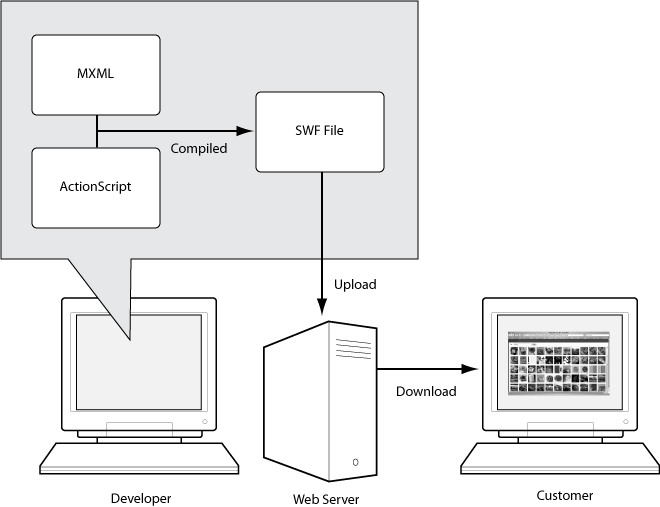
\includegraphics[width=7cm]{./images/as_to_swf}
\caption{\label{fig:as_to_swf} Proses kompilasi, \textit{deploy} dan akses aplikasi}
\end{center}
\end{figure}


%==========================================================================================================
% MULAI BAB IV
%==========================================================================================================
\chapter{PENGUJIAN DAN ANALISA}
\label{chap:pengujian}
%==========================================================================================================
% Subbab
%==========================================================================================================
Dalam pengujian aplikasi ini, ada dua cara pengujian yaitu dengan PC notebook yang dilengkapi \textit{webcam} internal atau menggunakan PC \textit{Desktop} dengan tambahan \textit{webcam}, konfigurasi sistem dapat dilihat pada gambar \ref{fig:monas_ar}. Untuk menjalankan aplikasi ini, diperlukan \textit{web browser} yang sudah terintegrasi \textit{plug-in} flash player versi 10. 

Spesifikasi sistem yang penulis gunakan dalam pengujian ini adalah sebagai berikut.
\begin{itemize}
\item Prosesor AMD Phenom\texttrademark II X4 955 Processor 3200 Mhz
\item Memori 2 Gb
\item standar usb 2.0 \textit{webcam} 
\item \textit{web browser} Mozilla Firefox versi 3.6.12
\end{itemize}

\begin{figure}[h]
\begin{center}
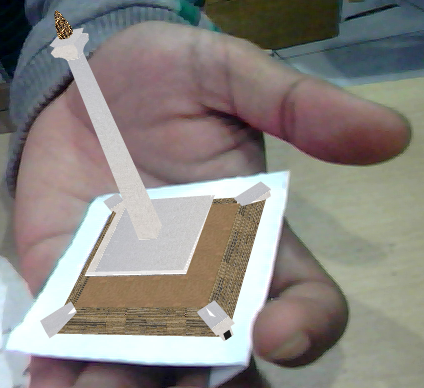
\includegraphics[width=6cm]{./images/ar3dv/monas_ar}
\caption{\label{fig:monas_ar} Hasil pengujian}
\end{center}
\end{figure}

Hasil pengujian dapat dilihat pada gambar \ref{fig:monas_ar}. Objek 3D dapat dirender dengan baik, meskipun kadang-kadang hilang dari marker, dikarenakan sistem tidak dapat menerima input dengan pergerakan yang marker cepat. Ada dua hal yang akan dianalisa yaitu fps (frame per second) dari video hasil rendering objek 3D dengan model yang berbeda-beda serta juga jarak dan sudut kemiringan marker yang masih dapat diterima aplikasi.

\section{Analisa \textit{Frame per Second (FPS)}}
\label{sec:analisa_fps}
\textit{Frame rate} atau frekuensi \textit{frame} merupakan frekuensi sebuah alat atau layar menghasilkan gambar yang disebut \textit{frame}. \textit{Frame rate} lebih sering dikenal dan diekspresikan sebagai frame per second (FPS). FPS merupakan jumlah gambar yang dihasilkan dalam waktu satu detik, mata manusia memerlukan jumlah \textit{frame} tertentu dalam satu detik agar dapat melihat gambar bergerak tanpa adanya \textit{flicker}. Jumlah FPS juga tergantung dari intensitas cahaya dan kecepatan objek bergerak dari video yang dihasilkan.

Pengujian untuk menganalisa FPS sangat diperlukan untuk mengetahui sejauh mana performa aplikasi viewer objek 3D ini. Untuk keperluan tersebut, penulis menambahkan informasi FPS tersebut ke aplikasi agar dapat dianalisa. Papervision3D telah menyediakan kelas untuk hal tersebut yaitu \textbf{StatsView}. Penggunaannya dapat dilihat dari \textit{listing} \ref{code:stats-view}.

\begin{lstlisting}[language=ActionScript,caption=StatsView,label=code:stats-view]
	_renderEngine = new LazyRenderEngine(_scene3D, _camera3D, _viewport3D);
	addChild(new StatsView(_renderEngine));
\end{lstlisting}

Sebuah informasi teks akan ditampilkan dikiri atas tampilan video, seperti yang ditunjukkan oleh gambar \ref{fig:fps_ar3dv}. Penulis menggunakan lima macam objek 3D berbeda dalam melakukan pengujian ini. Hasil pengujian dapat dilihat pada tabel \ref{tab:tabel_pengujian_fps}.

\begin{figure}[h]
\begin{center}
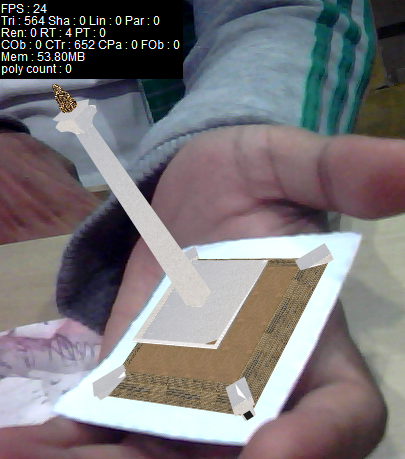
\includegraphics[width=6cm]{./images/ar3dv/monas_stats}
\caption{\label{fig:monas_stats} Hasil pengujian dengan statistik}
\end{center}
\end{figure}

\begin{table}[h]
\begin{center}
	\caption{Hasil Pengujian dengan Lima Model 3D}\label{tab:tabel_pengujian_fps}
	\vspace{5mm}
    \begin{tabular}[caption]{ | l | l | l | l | l | l | l |}
    \hline
    No & Nama & Tipe file & Ukuran file (KB) & FPS & Memory (MB) & Tri \cr \hline
    1 & airport & 3DS &  129,7 & 14 & 51,76 & 2870 \cr \hline
    2 & eiffel & DAE & 38,7 & 50 & 44,93 & 206 \cr \hline
	3 & monas & DAE & 154,5 & 24 & 53.80 & 564 \cr \hline
	4 & scout & DAE & 267,2 & 38 & 55.28 & 233 \cr \hline
	5 & tajmahal & DAE & 812,9 & 0 & 567.68 & 147.018 \cr \hline
    \hline
    \end{tabular}
\end{center}
\end{table}

Nilai FPS bergantung pada kompleksitas objek 3D yang ditampilkan. Untuk objek 3D yang tidak terlalu kompleks, hasilnya sangat baik, FPS berkisar antara 24 sampai 50, sehingga masih dapat terlihat baik. pada objek 3D kelima, nilai FPS nol atau tidak bergerak sama sekali, walaupun objek tersebut dapat terlihat. Penulis beranggapan bahwa frame yang dihasilkan dalam beberapa detik sekali, sehingga nilai FPS yang didapat adalah nol, hal ini disebabkan karena objek 3D yang di-\textit{render} sangat kompleks sehingga aplikasi tidak sanggup untum menampilkannya dengan baik.

%\section{Analisa Penggunaan Marker}
%\label{sec:analisa_marker}
%
%\subsection{Jarak}
%\label{subsec:analisa_jarak_marker}
%
%
%\subsection{Sudut Kemiringan}
%\label{subsec:analisa_sudut_marker}
%==========================================================================================================
% MULAI BAB V
%==========================================================================================================
\chapter{KESIMPULAN DAN SARAN}
\label{chap:penutup}
%==========================================================================================================
% Subbab
%==========================================================================================================
\section{Kesimpulan}
\label{sec:kesimpulan}
Berdasarkan pembahasan bab-bab sebelumnya dan didukung oleh hasil pengujian, dapat diambil kesimpulan sebagai berikut.
\begin{enumerate}
\item Aplikasi dapat berjalan dengan baik tanpa perlu menginstall aplikasinya, karena aplikasi diakses menggunakan browser yang mempunyai \textit{plug-in} flash. 
\item Aplikasi dapat merender objek 3D dengan format DAE dan 3DS sesuai dengan marker yang didteksi, akan tetapi tingkat pengenalan marker sangat dipengaruhi cahaya dan bentuk marker yang digunakan.
\item Aplikasi dapat merender objek 3D sederhana dengan baik dengan nilai FPS yang relatif baik (24 sampai 50). 
\item Untuk objek 3D kompleks aplikasi tidak dapat berjalan dengan baik, terjadi \textit{flicker} atau gambar tidak bergerak sama sekali.
\end{enumerate}

\section{Saran}
\label{sec:saran}
\begin{enumerate}
\item Untuk pengembangan selanjutnya, diharapkan dapat menggunakan \textit{library} yang lebih baik. Marker yang digunakan diharapkan lebih variatif, dengan pola yang lebih menarik atau mungkin dengan pola yang berwarna sehingga lebih menarik.
\item Perangkat keras yang digunakan tidak lagi komputer tapi berupa \textit{gadget} yang lebih kecil dan bisa menjalankan flash, sehingga aplikasi benar-benar dapat dijalankan dari mana saja. 
\end{enumerate}

%==========================================================================================================
% Bagian daftar pustaka 
%==========================================================================================================
\nocite{*}
\renewcommand{\bibname}{Daftar Pustaka}
\bibliographystyle{ieeetr} 
\bibliography{daftarpustaka}
\addcontentsline{toc}{chapter}{Daftar Pustaka} 

%==========================================================================================================
% MULAI BAGIAN LAMPIRAN
%==========================================================================================================
%\appendix % dengan menggunakan appendix nomor bab akan ditampilan dengan menggunakan huruf: menjadi Lampiran A
%\chapter{Listing Program} % contoh ini akan menampilkan bab baru yaitu Lampiran A - Data Pendukung 
\appendix

\chapter{\textit{Listing Source Code} Aplikasi}
\label{lampiran:listing_aplikasi}

\lstset{language=ActionScript,numbers=left}

\section{AR3DV.as}
\label{lampiran:AR3DV}
\lstinputlisting{./source_code/src/ar3dv/AR3DV.as}

\pagebreak

\section{AR3DVModelContainer.as}
\label{subsec:lampiran:AR3DVModelContainer}
\lstinputlisting{./source_code/src/ar3dv/AR3DVModelContainer.as}

\pagebreak
	
\section{AR3DVModel.as}
\label{lampiran:AR3DVModel}
\lstinputlisting{./source_code/src/ar3dv/AR3DVModel.as}

\pagebreak

\section{AR3DVModelEvent.as}
\label{lampiran:AR3DVModelEvent}
\lstinputlisting{./source_code/src/ar3dv/AR3DVModelEvent.as}

\pagebreak	
	
%\chapter{\textit{HTML Wrapper}}
%\label{chap:lampiran_HTML_Wrapper}

%\lstinputlisting[language=HTML]{../source_code/src/ar3dv/bin-debug/release/AR3DV.html}

\end{document}

